\documentclass[11pt]{article}

% Change "review" to "final" to generate the final (sometimes called camera-ready) version.
% Change to "preprint" to generate a non-anonymous version with page numbers.
\usepackage[preprint]{acl}

% Standard package includes
\usepackage{times}
\usepackage{latexsym}

% For proper rendering and hyphenation of words containing Latin characters (including in bib files)
\usepackage[T1]{fontenc}

% This assumes your files are encoded as UTF8
\usepackage[utf8]{inputenc}

% Improves layout and saves space
\usepackage{microtype}

% Improves aesthetics of typewriter font
\usepackage{inconsolata}

% Additional packages for math, tables, graphics, and Korean Hangul rendering
\usepackage{amsmath}
\usepackage{amssymb}
\usepackage{booktabs}
\usepackage{multirow}
\usepackage{array}
\usepackage{graphicx}
\usepackage{CJKutf8}
\usepackage{tikz}
\usepackage{pgfplots}
\pgfplotsset{compat=1.18}
\usetikzlibrary{arrows.meta,positioning,shapes.geometric,calc}

% Korean Hangul helper macro (renders UTF-8 Hangul via TeX Live CJKutf8 'mj' font)
\newcommand{\ko}[1]{\begin{CJK}{UTF8}{mj}#1\end{CJK}}

% Quotes
\usepackage{csquotes}

% Auto-generated experimental results macros
% Auto-generated by src/export_tex.py — DO NOT EDIT MANUALLY
% Update by running: python -m src.export_tex --results results/experiment_results.json

\newcommand{\qwenCBAccEN}{76.7}
\newcommand{\qwenCBAccKO}{56.0}
\newcommand{\qwenCBLcEN}{100.0}
\newcommand{\qwenCBLcKO}{100.0}
\newcommand{\qwenKnownBothN}{84}
\newcommand{\qwenKnownENOnlyN}{31}
\newcommand{\qwenKnownKOOnlyN}{0}
\newcommand{\qwenUnknownBothN}{35}
\newcommand{\qwenMonoAccEN}{86.7}
\newcommand{\qwenMonoOverrideEN}{13.3}
\newcommand{\qwenMonoFirstDocEN}{56.0}
\newcommand{\qwenMonoAbstainEN}{1.7}
\newcommand{\qwenMonoLCEN}{100.0}
\newcommand{\qwenMonoAccKO}{81.3}
\newcommand{\qwenMonoOverrideKO}{18.7}
\newcommand{\qwenMonoFirstDocKO}{62.7}
\newcommand{\qwenMonoAbstainKO}{2.0}
\newcommand{\qwenMonoLCKO}{100.0}
\newcommand{\qwenMonoAccAll}{84.0}
\newcommand{\qwenMonoOverrideAll}{16.0}
\newcommand{\qwenMonoFirstDocAll}{59.3}
\newcommand{\qwenMonoAbstainAll}{1.8}
\newcommand{\qwenMonoLCAll}{100.0}
\newcommand{\qwenEPREN}{90.3}
\newcommand{\qwenEPRLPEN}{90.3}
\newcommand{\qwenEPRTxtEN}{90.0}
\newcommand{\qwenEPRCILowEN}{87.7}
\newcommand{\qwenEPRCIHighEN}{92.4}
\newcommand{\qwenFlipABRateEN}{81.0}
\newcommand{\qwenFlipBARateEN}{0.3}
\newcommand{\qwenTruthAARateEN}{18.7}
\newcommand{\qwenFalseBBRateEN}{0.0}
\newcommand{\qwenFlipABNEN}{243}
\newcommand{\qwenFlipBANEN}{1}
\newcommand{\qwenTruthAANEN}{56}
\newcommand{\qwenFalseBBNEN}{0}
\newcommand{\qwenCondENFlipEN}{99.6}
\newcommand{\qwenMcNemarChiEN}{238.0}
\newcommand{\qwenMcNemarPEN}{<0.0001}
\newcommand{\qwenFactAccEN}{59.3}
\newcommand{\qwenPairOneAccEN}{99.7}
\newcommand{\qwenPairTwoOverrideEN}{81.0}
\newcommand{\qwenFirstDocEN}{53.0}
\newcommand{\qwenAbstainEN}{3.3}
\newcommand{\qwenLCEN}{100.0}
\newcommand{\qwenLPShiftMeanEN}{0.97}
\newcommand{\qwenLPShiftTEN}{42.8}
\newcommand{\qwenEPRKO}{67.0}
\newcommand{\qwenEPRLPKO}{67.0}
\newcommand{\qwenEPRTxtKO}{67.7}
\newcommand{\qwenEPRCILowKO}{63.1}
\newcommand{\qwenEPRCIHighKO}{70.6}
\newcommand{\qwenFlipABRateKO}{41.7}
\newcommand{\qwenFlipBARateKO}{7.7}
\newcommand{\qwenTruthAARateKO}{44.7}
\newcommand{\qwenFalseBBRateKO}{6.0}
\newcommand{\qwenFlipABNKO}{125}
\newcommand{\qwenFlipBANKO}{23}
\newcommand{\qwenTruthAANKO}{134}
\newcommand{\qwenFalseBBNKO}{18}
\newcommand{\qwenCondENFlipKO}{84.5}
\newcommand{\qwenMcNemarChiKO}{68.9}
\newcommand{\qwenMcNemarPKO}{<0.0001}
\newcommand{\qwenFactAccKO}{69.3}
\newcommand{\qwenPairOneAccKO}{86.3}
\newcommand{\qwenPairTwoOverrideKO}{47.7}
\newcommand{\qwenFirstDocKO}{59.7}
\newcommand{\qwenAbstainKO}{2.0}
\newcommand{\qwenLCKO}{96.8}
\newcommand{\qwenLPShiftMeanKO}{0.30}
\newcommand{\qwenLPShiftTKO}{12.8}
\newcommand{\qwenEPRAll}{78.7}
\newcommand{\qwenEPRLPAll}{78.7}
\newcommand{\qwenEPRTxtAll}{78.7}
\newcommand{\qwenEPRCILowAll}{76.3}
\newcommand{\qwenEPRCIHighAll}{80.9}
\newcommand{\qwenFlipABRateAll}{61.3}
\newcommand{\qwenFlipBARateAll}{4.0}
\newcommand{\qwenTruthAARateAll}{31.7}
\newcommand{\qwenFalseBBRateAll}{3.0}
\newcommand{\qwenFlipABNAll}{368}
\newcommand{\qwenFlipBANAll}{24}
\newcommand{\qwenTruthAANAll}{190}
\newcommand{\qwenFalseBBNAll}{18}
\newcommand{\qwenCondENFlipAll}{93.9}
\newcommand{\qwenMcNemarChiAll}{300.1}
\newcommand{\qwenMcNemarPAll}{<0.0001}
\newcommand{\qwenFactAccAll}{64.3}
\newcommand{\qwenPairOneAccAll}{93.0}
\newcommand{\qwenPairTwoOverrideAll}{64.3}
\newcommand{\qwenFirstDocAll}{56.3}
\newcommand{\qwenAbstainAll}{2.7}
\newcommand{\qwenLCAll}{98.4}
\newcommand{\qwenLPShiftMeanAll}{0.63}
\newcommand{\qwenLPShiftTAll}{29.9}
\newcommand{\qwenPKKnownBothEPRAll}{76.9}
\newcommand{\qwenPKKnownBothEPREN}{88.7}
\newcommand{\qwenPKKnownBothEPRKO}{65.2}
\newcommand{\qwenPKKnownBothOverrideAll}{57.4}
\newcommand{\qwenPKKnownBothFactAccAll}{69.5}
\newcommand{\qwenPKKnownENOnlyEPRAll}{80.6}
\newcommand{\qwenPKKnownENOnlyEPREN}{91.1}
\newcommand{\qwenPKKnownENOnlyEPRKO}{70.2}
\newcommand{\qwenPKKnownENOnlyOverrideAll}{70.2}
\newcommand{\qwenPKKnownENOnlyFactAccAll}{60.5}
\newcommand{\qwenPKUnknownBothEPRAll}{81.1}
\newcommand{\qwenPKUnknownBothEPREN}{93.6}
\newcommand{\qwenPKUnknownBothEPRKO}{68.6}
\newcommand{\qwenPKUnknownBothOverrideAll}{75.7}
\newcommand{\qwenPKUnknownBothFactAccAll}{55.4}
\newcommand{\qwenPKAnyKnownEPRAll}{77.9}
\newcommand{\qwenPKAnyKnownEPREN}{89.3}
\newcommand{\qwenPKAnyKnownEPRKO}{66.5}
\newcommand{\qwenPKAnyKnownOverrideAll}{60.9}
\newcommand{\qwenPKAnyKnownFactAccAll}{67.1}
\newcommand{\qwenCatEntityEPRAll}{81.0}
\newcommand{\qwenCatEntityEPREN}{91.5}
\newcommand{\qwenCatEntityEPRKO}{70.5}
\newcommand{\qwenCatEntityLCKO}{90.5}
\newcommand{\qwenCatEntityFlipABAll}{65.0}
\newcommand{\qwenCatDateEPRAll}{78.2}
\newcommand{\qwenCatDateEPREN}{93.0}
\newcommand{\qwenCatDateEPRKO}{63.5}
\newcommand{\qwenCatDateLCKO}{100.0}
\newcommand{\qwenCatDateFlipABAll}{60.0}
\newcommand{\qwenCatNumberEPRAll}{76.8}
\newcommand{\qwenCatNumberEPREN}{86.5}
\newcommand{\qwenCatNumberEPRKO}{67.0}
\newcommand{\qwenCatNumberLCKO}{100.0}
\newcommand{\qwenCatNumberFlipABAll}{59.0}
\newcommand{\qwenOrdENFirstEPRAll}{85.0}
\newcommand{\qwenOrdENFirstEPREN}{93.3}
\newcommand{\qwenOrdENFirstEPRKO}{76.7}
\newcommand{\qwenOrdKOFirstEPRAll}{72.3}
\newcommand{\qwenOrdKOFirstEPREN}{87.3}
\newcommand{\qwenOrdKOFirstEPRKO}{57.3}
\newcommand{\llamaCBAccEN}{73.3}
\newcommand{\llamaCBAccKO}{35.3}
\newcommand{\llamaCBLcEN}{100.0}
\newcommand{\llamaCBLcKO}{100.0}
\newcommand{\llamaKnownBothN}{53}
\newcommand{\llamaKnownENOnlyN}{57}
\newcommand{\llamaKnownKOOnlyN}{0}
\newcommand{\llamaUnknownBothN}{40}
\newcommand{\llamaMonoAccEN}{88.3}
\newcommand{\llamaMonoOverrideEN}{11.7}
\newcommand{\llamaMonoFirstDocEN}{57.7}
\newcommand{\llamaMonoAbstainEN}{2.0}
\newcommand{\llamaMonoLCEN}{100.0}
\newcommand{\llamaMonoAccKO}{74.0}
\newcommand{\llamaMonoOverrideKO}{26.0}
\newcommand{\llamaMonoFirstDocKO}{64.0}
\newcommand{\llamaMonoAbstainKO}{2.0}
\newcommand{\llamaMonoLCKO}{100.0}
\newcommand{\llamaMonoAccAll}{81.2}
\newcommand{\llamaMonoOverrideAll}{18.8}
\newcommand{\llamaMonoFirstDocAll}{60.8}
\newcommand{\llamaMonoAbstainAll}{2.0}
\newcommand{\llamaMonoLCAll}{100.0}
\newcommand{\llamaEPREN}{92.8}
\newcommand{\llamaEPRLPEN}{92.8}
\newcommand{\llamaEPRTxtEN}{92.9}
\newcommand{\llamaEPRCILowEN}{90.5}
\newcommand{\llamaEPRCIHighEN}{94.6}
\newcommand{\llamaFlipABRateEN}{85.7}
\newcommand{\llamaFlipBARateEN}{0.0}
\newcommand{\llamaTruthAARateEN}{14.0}
\newcommand{\llamaFalseBBRateEN}{0.3}
\newcommand{\llamaFlipABNEN}{257}
\newcommand{\llamaFlipBANEN}{0}
\newcommand{\llamaTruthAANEN}{42}
\newcommand{\llamaFalseBBNEN}{1}
\newcommand{\llamaCondENFlipEN}{100.0}
\newcommand{\llamaMcNemarChiEN}{255.0}
\newcommand{\llamaMcNemarPEN}{<0.0001}
\newcommand{\llamaFactAccEN}{56.8}
\newcommand{\llamaPairOneAccEN}{99.7}
\newcommand{\llamaPairTwoOverrideEN}{86.0}
\newcommand{\llamaFirstDocEN}{51.5}
\newcommand{\llamaAbstainEN}{2.8}
\newcommand{\llamaLCEN}{100.0}
\newcommand{\llamaLPShiftMeanEN}{1.08}
\newcommand{\llamaLPShiftTEN}{45.1}
\newcommand{\llamaEPRKO}{84.7}
\newcommand{\llamaEPRLPKO}{84.7}
\newcommand{\llamaEPRTxtKO}{85.1}
\newcommand{\llamaEPRCILowKO}{81.6}
\newcommand{\llamaEPRCIHighKO}{87.3}
\newcommand{\llamaFlipABRateKO}{71.3}
\newcommand{\llamaFlipBARateKO}{2.0}
\newcommand{\llamaTruthAARateKO}{21.7}
\newcommand{\llamaFalseBBRateKO}{5.0}
\newcommand{\llamaFlipABNKO}{214}
\newcommand{\llamaFlipBANKO}{6}
\newcommand{\llamaTruthAANKO}{65}
\newcommand{\llamaFalseBBNKO}{15}
\newcommand{\llamaCondENFlipKO}{97.3}
\newcommand{\llamaMcNemarChiKO}{194.8}
\newcommand{\llamaMcNemarPKO}{<0.0001}
\newcommand{\llamaFactAccKO}{58.3}
\newcommand{\llamaPairOneAccKO}{93.0}
\newcommand{\llamaPairTwoOverrideKO}{76.3}
\newcommand{\llamaFirstDocKO}{56.7}
\newcommand{\llamaAbstainKO}{2.3}
\newcommand{\llamaLCKO}{94.2}
\newcommand{\llamaLPShiftMeanKO}{0.62}
\newcommand{\llamaLPShiftTKO}{29.2}
\newcommand{\llamaEPRAll}{88.8}
\newcommand{\llamaEPRLPAll}{88.8}
\newcommand{\llamaEPRTxtAll}{89.0}
\newcommand{\llamaEPRCILowAll}{86.8}
\newcommand{\llamaEPRCIHighAll}{90.4}
\newcommand{\llamaFlipABRateAll}{78.5}
\newcommand{\llamaFlipBARateAll}{1.0}
\newcommand{\llamaTruthAARateAll}{17.8}
\newcommand{\llamaFalseBBRateAll}{2.7}
\newcommand{\llamaFlipABNAll}{471}
\newcommand{\llamaFlipBANAll}{6}
\newcommand{\llamaTruthAANAll}{107}
\newcommand{\llamaFalseBBNAll}{16}
\newcommand{\llamaCondENFlipAll}{98.7}
\newcommand{\llamaMcNemarChiAll}{451.4}
\newcommand{\llamaMcNemarPAll}{<0.0001}
\newcommand{\llamaFactAccAll}{57.6}
\newcommand{\llamaPairOneAccAll}{96.3}
\newcommand{\llamaPairTwoOverrideAll}{81.2}
\newcommand{\llamaFirstDocAll}{54.1}
\newcommand{\llamaAbstainAll}{2.6}
\newcommand{\llamaLCAll}{97.1}
\newcommand{\llamaLPShiftMeanAll}{0.85}
\newcommand{\llamaLPShiftTAll}{45.8}
\newcommand{\llamaPKKnownBothEPRAll}{84.2}
\newcommand{\llamaPKKnownBothEPREN}{89.6}
\newcommand{\llamaPKKnownBothEPRKO}{78.8}
\newcommand{\llamaPKKnownBothOverrideAll}{68.4}
\newcommand{\llamaPKKnownBothFactAccAll}{65.8}
\newcommand{\llamaPKKnownENOnlyEPRAll}{90.4}
\newcommand{\llamaPKKnownENOnlyEPREN}{92.5}
\newcommand{\llamaPKKnownENOnlyEPRKO}{88.2}
\newcommand{\llamaPKKnownENOnlyOverrideAll}{86.4}
\newcommand{\llamaPKKnownENOnlyFactAccAll}{53.9}
\newcommand{\llamaPKUnknownBothEPRAll}{92.5}
\newcommand{\llamaPKUnknownBothEPREN}{97.5}
\newcommand{\llamaPKUnknownBothEPRKO}{87.5}
\newcommand{\llamaPKUnknownBothOverrideAll}{90.6}
\newcommand{\llamaPKUnknownBothFactAccAll}{51.9}
\newcommand{\llamaPKAnyKnownEPRAll}{87.4}
\newcommand{\llamaPKAnyKnownEPREN}{91.1}
\newcommand{\llamaPKAnyKnownEPRKO}{83.6}
\newcommand{\llamaPKAnyKnownOverrideAll}{77.7}
\newcommand{\llamaPKAnyKnownFactAccAll}{59.7}
\newcommand{\llamaCatEntityEPRAll}{90.8}
\newcommand{\llamaCatEntityEPREN}{94.5}
\newcommand{\llamaCatEntityEPRKO}{87.0}
\newcommand{\llamaCatEntityLCKO}{82.5}
\newcommand{\llamaCatEntityFlipABAll}{81.5}
\newcommand{\llamaCatDateEPRAll}{88.0}
\newcommand{\llamaCatDateEPREN}{91.5}
\newcommand{\llamaCatDateEPRKO}{84.5}
\newcommand{\llamaCatDateLCKO}{100.0}
\newcommand{\llamaCatDateFlipABAll}{77.5}
\newcommand{\llamaCatNumberEPRAll}{87.5}
\newcommand{\llamaCatNumberEPREN}{92.5}
\newcommand{\llamaCatNumberEPRKO}{82.5}
\newcommand{\llamaCatNumberLCKO}{100.0}
\newcommand{\llamaCatNumberFlipABAll}{76.5}
\newcommand{\llamaOrdENFirstEPRAll}{92.8}
\newcommand{\llamaOrdENFirstEPREN}{94.3}
\newcommand{\llamaOrdENFirstEPRKO}{91.3}
\newcommand{\llamaOrdKOFirstEPRAll}{84.7}
\newcommand{\llamaOrdKOFirstEPREN}{91.3}
\newcommand{\llamaOrdKOFirstEPRKO}{78.0}


\title{Language Bias in Conflicting Multilingual RAG Evidence}

\author{Alan Mattia Cantekin \\
  Hanyang University / 222 Wangsimni-ro, Seongdong-gu, Seoul, South Korea \\
  \texttt{iacantek@hanyang.ac.kr} \\
}

\begin{document}
\maketitle

\begin{abstract}
Multilingual Retrieval-Augmented Generation (mRAG) systems frequently retrieve documents in multiple languages simultaneously. Because web corpora vary in coverage and recency across languages, high-resource English passages and lower-resource non-English passages can assert mutually exclusive factual claims. While prior studies examine language bias in retrieval, reranking, or citation selection over complementary passages, how large language models (LLMs) resolve direct cross-lingual factual contradictions remains unexplored. We introduce a counterbalanced evaluation protocol on a 150-item English--Korean benchmark derived from MKQA (\textsc{MKQA-Conflict-150}), spanning 50 named entities, 50 dates, and 50 numeric facts ($2{,}100$ inference runs per model). For each query, we pair ground-truth claim $A$ against a type-matched counterfactual $B$ across swapped language assignments ($\text{Pair}_1$: $[\text{EN}{=}A, \text{KO}{=}B]$ vs.\ $\text{Pair}_2$: $[\text{KO}{=}A, \text{EN}{=}B]$), crossed with query language and passage order. Evaluating \texttt{Qwen-2.5-7B-Instruct} and \texttt{Llama-3.1-8B-Instruct} via exact extraction and concept-marginalized log-probabilities reveals a strong English authority bias: overall English Preference Rate (EPR) reaches \qwenEPRAll\% for Qwen and \llamaEPRAll\% for Llama ($p \qwenMcNemarPAll$). Crucially, when the English passage asserts a falsehood against a truthful Korean passage ($\text{Pair}_2$), models override factual truth in \qwenPairTwoOverrideAll\% and \llamaPairTwoOverrideAll\% of cases, even when the fact is known parametrically.
\end{abstract}


\section{Introduction}
\label{sec:intro}

Retrieval-Augmented Generation (RAG) grounds large language models (LLMs) in external evidence to mitigate hallucination and update stale parametric memory \citep{lewis2020retrieval,karpukhin2020dense}. In multilingual settings (mRAG), users issue queries in local languages while retrieval spans a global multi-language index \citep{asai2021xor,asai2021one,chirkova2024retrieval}. Because web corpora are heavily skewed toward English, cross-lingual retrieval is indispensable for answering non-English queries \citep{wu2024not,liu2025xrag}. Yet retrieving evidence across languages introduces a critical vulnerability: \emph{cross-lingual factual contradiction}. In real-world mRAG pipelines, an English passage and a local-language passage (e.g., Korean) retrieved for the same query frequently assert mutually exclusive facts due to asynchronous updates, translation errors, or corpus-specific misinformation.

Understanding how LLMs adjudicate direct cross-lingual contradictions is vital for trustworthy mRAG deployment. If a generator systematically treats English context as more authoritative than non-English context regardless of factual validity, an outdated or false English passage will overwrite an accurate local-language passage---a failure mode we term \emph{cross-lingual truth override}. Conversely, if a generator exhibits rigid query-language nepotism \citep{ki2025}, it may copy a false local-language claim while ignoring corrective English evidence. Either bias degrades factual reliability and creates epistemic disparities across language communities \citep{sharma2025faux,chataigner2025multilingual}.

Isolating document-language bias during conflict resolution is challenging because three confounders co-occur in standard mRAG evaluation: (1) asymmetric \emph{parametric prior knowledge}, as LLMs recall facts more reliably in English than in lower-resource languages \citep{qi2023crosslingual,wang2025lost}; (2) \emph{passage position sensitivity} \citep{liu2024lost}, which confounds language preference if one language is ranked higher by the retriever; and (3) surface \emph{script attraction} or decoding-time language drift when named entities appear in distinct scripts (Latin vs.\ Korean Hangul; \citealp{li2025}).

\begin{figure*}[t]
\centering
\resizebox{\textwidth}{!}{%
\begin{tikzpicture}[
    font=\footnotesize,
    box/.style={draw=black!75, rounded corners=3pt, thick, align=left, inner sep=4pt, fill=white},
    enbox/.style={draw=blue!70!black, rounded corners=3pt, thick, align=left, inner sep=4pt, fill=blue!4},
    kobox/.style={draw=teal!75!black, rounded corners=3pt, thick, align=left, inner sep=4pt, fill=teal!4},
    regime/.style={draw=black!70, rounded corners=2.5pt, semithick, align=center, inner sep=3pt, fill=gray!6},
    arrow/.style={-{Stealth[length=2.0mm,width=1.5mm]}, thick, draw=black!75}
]
% Left column: Query & Fact Pair
\node[box, text width=4.3cm] (query) at (0, 0) {
  \textbf{MKQA Query $q(\ell_q)$} ($\ell_q \in \{\text{EN}, \text{KO}\}$)\\[1pt]
  \textbf{EN:} \emph{``who produces the most pistachios in the world?''}\\
  \textbf{KO:} \ko{전 세계에서 누가 가장 많은 피스타치오를 생산하나요}\\
  \scriptsize\emph{(jeon segye-eseo nuga gajang manh-eun piseutachio-reul saengsanhanayo)}\\[1.5pt]
  \footnotesize\textbf{True $A$:} \texttt{Iran} / \ko{이란} \emph{(iran)}\\
  \textbf{False $B$:} \texttt{Turkey} / \ko{터키} \emph{(teoki)}
};

% Middle column: Counterbalanced Pairs
\node[enbox, text width=6.3cm] (pair1) at (6.25, 1.08) {
  \textbf{Condition $\text{Pair}_1$: $[\text{EN}{=}A,\; \text{KO}{=}B]$} \hfill \scriptsize(2 orders: EN/KO-first)\\[1pt]
  $\bullet$ $d_{\text{en}}(A)$: \emph{``The country that produces the most pistachios in the world is \textbf{Iran}.''}\\
  $\bullet$ $d_{\text{ko}}(B)$: \ko{전 세계에서 피스타치오를 가장 많이 생산하는 국가는 \textbf{터키}이다.} \scriptsize\emph{(...gukga-neun \textbf{teoki}-ida.)}
};

\node[kobox, text width=6.3cm] (pair2) at (6.25, -1.08) {
  \textbf{Condition $\text{Pair}_2$: $[\text{KO}{=}A,\; \text{EN}{=}B]$} \hfill \scriptsize(2 orders: EN/KO-first)\\[1pt]
  $\bullet$ $d_{\text{ko}}(A)$: \ko{전 세계에서 피스타치오를 가장 많이 생산하는 국가는 \textbf{이란}이다.} \scriptsize\emph{(...gukga-neun \textbf{iran}-ida.)}\\
  $\bullet$ $d_{\text{en}}(B)$: \emph{``The country that produces the most pistachios in the world is \textbf{Turkey}.''}
};

% LLM Node
\node[box, text width=2.2cm, align=center, fill=orange!8, draw=orange!70!black] (llm) at (11.55, 0) {
  \textbf{mRAG}\\
  \textbf{Generator}\\[1pt]
  \scriptsize Qwen-2.5-7B\\[-1pt]
  \scriptsize Llama-3.1-8B\\[1.5pt]
  \scriptsize Dual Scoring:\\[-1pt]
  \scriptsize Exact + $\ell_{\text{concept}}$
};

% Right column: 4 Regimes (compact 2-line boxes with crisp vertical spacing)
\node[regime, text width=4.3cm, fill=red!7, draw=red!65!black] (r1) at (15.85, 1.60) {
  \textbf{English Flip $(y_1{=}A \to y_2{=}B)$}\\
  \scriptsize Follows $\text{EN}$ doc (overrides truth in $\text{Pair}_2$)
};
\node[regime, text width=4.3cm, fill=teal!8, draw=teal!65!black] (r2) at (15.85, 0.53) {
  \textbf{Korean Flip $(y_1{=}B \to y_2{=}A)$}\\
  \scriptsize Follows $\text{KO}$ doc (overrides truth in $\text{Pair}_1$)
};
\node[regime, text width=4.3cm, fill=green!7, draw=green!55!black] (r3) at (15.85, -0.53) {
  \textbf{Truth-Consistent $(y_1{=}A \to y_2{=}A)$}\\
  \scriptsize Retains ground-truth $A$ in both pairs
};
\node[regime, text width=4.3cm, fill=gray!10, draw=black!50] (r4) at (15.85, -1.60) {
  \textbf{False-Consistent $(y_1{=}B \to y_2{=}B)$}\\
  \scriptsize Selects counterfactual $B$ in both pairs
};

% Arrows
\draw[arrow] (query.east) -- ++(0.35,0) |- (pair1.west);
\draw[arrow] (query.east) -- ++(0.35,0) |- (pair2.west);
\draw[arrow] (pair1.east) -- ++(0.35,0) |- ([yshift=2.5mm]llm.west);
\draw[arrow] (pair2.east) -- ++(0.35,0) |- ([yshift=-2.5mm]llm.west);
\draw[arrow] ([yshift=3.5mm]llm.east) -- ++(0.35,0) |- (r1.west);
\draw[arrow] ([yshift=1.2mm]llm.east) -- ++(0.35,0) |- (r2.west);
\draw[arrow] ([yshift=-1.2mm]llm.east) -- ++(0.35,0) |- (r3.west);
\draw[arrow] ([yshift=-3.5mm]llm.east) -- ++(0.35,0) |- (r4.west);
\end{tikzpicture}%
}
\vspace{-6pt}
\caption{Overview of our counterbalanced cross-lingual conflict protocol. Each item pairs ground-truth claim $A$ against a type-matched counterfactual $B$ across swapped language assignments ($\text{Pair}_1$ vs.\ $\text{Pair}_2$), two query languages ($\text{EN}$, $\text{KO}$), and two passage orders. Comparing paired decisions $(y_1, y_2) \in \{A,B\}^2$ isolates English document preference ($A \to B$) and Korean document preference ($B \to A$) from parametric truth retention ($A \to A$).}
\label{fig:protocol}
\vspace{-8pt}
\end{figure*}

Prior mRAG studies have not isolated how generators resolve direct cross-lingual factual contradictions. Existing work measures language bias in \emph{retrieval and reranking} \citep{park2025,wang2026}, evaluates \emph{distractor-based} context utilization where non-gold passages lack an answer \citep{qi2025}, characterizes \emph{decoding-time language drift} under non-conflicting evidence \citep{li2025}, or studies \emph{in-line citation selection} (\texttt{[1]}--\texttt{[9]}) across parallel or complementary documents without testing which claim the generator believes under direct contradiction \citep{ki2025}.

To bridge this gap, we introduce a counterbalanced framework (Figure~\ref{fig:protocol}) on 150 culturally neutral questions from MKQA \citep{longpre2021mkqa} balanced across named entities, dates, and numbers (\textsc{MKQA-Conflict-150}). Embedding true claim $A$ and counterfactual $B$ into parallel declarative templates with automatic Korean particle resolution across swapped language--claim assignments ($\text{Pair}_1: [\text{EN}{=}A, \text{KO}{=}B]$ vs.\ $\text{Pair}_2: [\text{KO}{=}A, \text{EN}{=}B]$), query languages, and passage orders decouples language bias from parametric memory and position bias. We test three hypotheses:
\begin{itemize}\setlength{\itemsep}{0pt}\setlength{\parskip}{0pt}\setlength{\topsep}{1pt}
    \item \textbf{$\mathcal{H}_{\text{EN}}$ (English Authority):} Generators assign higher epistemic weight to English context, yielding an English Preference Rate ($\text{EPR}$) $> 50\%$ across both query languages and high truth override ($A \to B$) when English is false.
    \item \textbf{$\mathcal{H}_{\text{QL}}$ (Query-Language Alignment):} Generators exhibit query--document nepotism \citep{ki2025}, favoring English on English queries ($\text{EPR}_{\text{EN}} > 50\%$) but reversing preference toward Korean on Korean queries ($\text{EPR}_{\text{KO}} < 50\%$).
    \item \textbf{$\mathcal{H}_{\text{Prior}}$ (Parametric Truth Retention):} When a fact is known in closed-book memory, internal priors anchor generation to truth $A$ regardless of context language ($A \to A$), driving $\text{EPR} \to 50\%$.
\end{itemize}
Evaluating \texttt{Qwen-2.5-7B-Instruct} \citep{yang2024qwen25} and \texttt{Llama-3.1-8B-Instruct} \citep{grattafiori2024llama3} across $4{,}200$ runs confirms $\mathcal{H}_{\text{EN}}$: overall $\text{EPR}$ reaches \qwenEPRAll\% for Qwen and \llamaEPRAll\% for Llama ($p \qwenMcNemarPAll$). Even on Korean queries, $\text{EPR}_{\text{KO}}$ remains \qwenEPRKO\% and \llamaEPRKO\%, refuting a reversal under $\mathcal{H}_{\text{QL}}$, and false English passages override true Korean passages in \qwenPairTwoOverrideAll\% and \llamaPairTwoOverrideAll\% of $\text{Pair}_2$ runs.


\section{Related Work}
\label{sec:related_work}

\subsection{Language Bias in Retrieval and Reranking}
\label{subsec:rw_retrieval}

Cross-lingual open-retrieval QA links non-English queries to multilingual collections \citep{asai2021xor,asai2021one,asai2022mia,zhang2023miracl}, yet retrieval fairness across languages remains uneven \citep{yang2024language,amiraz2025crosslingual}. \citet{park2025} measured language preference across mRAG retrieval and generation via Mean Language Rank Shift (MLRS) on MKQA \citep{longpre2021mkqa} and BordIRLines \citep{li2024bordirlines}, showing that dense retrievers favor same-language and Latin-script passages while generator outputs align in LaBSE embedding space with high-resource contexts. However, \citet{park2025} evaluated generators only over fixed top-$k$ mixtures or uniform single-language translations, never pitting two languages against each other on mutually exclusive claims. Recently, \citet{wang2026} showed that neural rerankers filter out lower-resource passages, leaving a 12--18 point recall gap below an oracle reranker on Korean MKQA queries. Their distilled reranker, LAURA, improved 10 of 13 languages, yet Korean was the only language where LAURA failed to improve accuracy ($25.0\%$ vs.\ $24.8\%, p{=}0.498$). Our work complements \citet{park2025} and \citet{wang2026} by isolating what happens \emph{inside the generator} when conflicting English and Korean passages both reach the context window.

\subsection{Generator Utilization and Linguistic Nepotism}
\label{subsec:rw_generator}

Studies of multilingual context utilization \citep{chirkova2024retrieval,wu2024not,liu2025xrag} show substantial cross-lingual performance gaps. \citet{qi2025} introduced \textsc{GMMLU-Choice} across 15 languages, showing via option log-likelihoods that LLMs comprehend non-English gold passages nearly as well as English passages when free-form generation bottlenecks are removed. Yet their non-gold passages were topically related distractors that \emph{contained no competing answer}. Closest to our study, \citet{ki2025} coined \emph{linguistic nepotism} to describe a generator's preference for citing documents in the query language. Using parallel passages from GlobalVoices and relevant-versus-irrelevant pairs on MIRACL \citep{zhang2023miracl}, \citet{ki2025} found that English queries cite English passages $66\%$--$98\%$ of the time while non-English queries preferentially cite query-language passages. However, \citet{ki2025} evaluated \emph{in-line citation indices} (\texttt{[1]}--\texttt{[9]}) over parallel translations, complementary facts, or irrelevant distractors rather than conflicting claims. Our counterbalanced protocol tests whether query-language nepotism ($\mathcal{H}_{\text{QL}}$) or English authority ($\mathcal{H}_{\text{EN}}$) prevails under direct factual contradiction.

\subsection{Latent English Dominance and Language Drift}
\label{subsec:rw_drift}

Multilingual transformers process non-English inputs through intermediate representations anchored to English \citep{wendler2024llamas}, often causing \emph{language drift} into the retrieved passage's language during decoding \citep{chirkova2024retrieval,wu2024not}. \citet{li2025} distinguished reasoning-initialization drift from entity-Continuum drift triggered after generating cross-lingual named entities. Extending \citet{li2025}, we test whether latent English dominance also drives generators to trust English factual claims over Korean claims, and whether Latin-versus-Hangul script divergence amplifies this bias relative to shared Arabic numerals.

\subsection{Cross-Lingual Factual Consistency and Conflicts}
\label{subsec:rw_consistency}

Multilingual LMs frequently return inconsistent closed-book answers across languages \citep{fierro2022factual,qi2023crosslingual,wang2025lost}, creating cross-lingual hallucination gaps \citep{sharma2025faux,chataigner2025multilingual}. In geopolitically disputed domains such as BordIRLines \citep{li2024bordirlines,li2025culturally}, Wikipedia editions naturally conflict, motivating dialectic prompting \citep{ranaldi2025improving}. Because cultural disputes entangle language bias with cultural priors, we restrict \textsc{MKQA-Conflict-150} to culturally neutral facts and counterbalance language--claim assignments.


\section{Method}
\label{sec:method}

To measure generator-level language preference under direct factual contradiction without confounding from parametric memory, passage position, or surface morphosyntax, we design a counterbalanced cross-lingual conflict protocol paired with dual discrete-and-probabilistic scoring.

\subsection{Problem Formulation and Notation}
\label{subsec:formulation}

Let $\mathcal{D} = \{e_1, \dots, e_N\}$ denote a benchmark of $N{=}150$ culturally neutral factual items partitioned equally into three categories: named entities ($\textsc{Entity}$), calendar years ($\textsc{Date}$), and numeric quantities ($\textsc{Number}$). Each item $e_i$ consists of: (1) parallel queries $q_i(\text{en})$ in English and $q_i(\text{ko})$ in Korean asking for the same atomic fact; (2) a ground-truth concept $A_i = (a_{i,\text{en}}, a_{i,\text{ko}})$ and a plausible, type-matched counterfactual $B_i = (b_{i,\text{en}}, b_{i,\text{ko}})$, where $\textsc{Entity}$ items contrast Latin script ($a_{i,\text{en}}, b_{i,\text{en}}$) with Hangul ($a_{i,\text{ko}}, b_{i,\text{ko}}$) while $\textsc{Date}$ and $\textsc{Number}$ share identical Arabic numerals ($a_{i,\text{en}}{=}a_{i,\text{ko}}$, $b_{i,\text{en}}{=}b_{i,\text{ko}}$); and (3) parallel declarative templates $T_{i,\text{en}}(\cdot)$ and $T_{i,\text{ko}}(\cdot)$ embedding any candidate $C \in \{A_i, B_i\}$ into an equivalent assertion $d_{\text{en}}(C) = T_{i,\text{en}}(c_{\text{en}})$ and $d_{\text{ko}}(C) = T_{i,\text{ko}}(c_{\text{ko}})$. Given a prompt $x$ with query $q_i(\ell_q)$ ($\ell_q \in \{\text{en}, \text{ko}\}$) and ordered context documents $(D_1, D_2)$ asserting competing claims $A_i$ and $B_i$, the generator outputs decision $y(x) \in \{A, B\}$.

\subsection{Counterbalanced Cross-Lingual Conflict Protocol}
\label{subsec:protocol}

In a naive test where English always asserts $A_i$ and Korean always asserts $B_i$, choosing $A_i$ conflates English preference with closed-book recall of truth $A_i$. We eliminate this confound by evaluating every item $e_i$ under two counterbalanced assignments:
\begin{equation}
\footnotesize
\text{Pair}_{i,1}\!:\! \{d_{\text{en}}(A_i), d_{\text{ko}}(B_i)\},\;
\text{Pair}_{i,2}\!:\! \{d_{\text{ko}}(A_i), d_{\text{en}}(B_i)\}.
\label{eq:pairs}
\end{equation}
To control for query-language alignment and position bias, we cross $\{\text{Pair}_{i,1}, \text{Pair}_{i,2}\}$ with query languages $\ell_q \in \{\text{en}, \text{ko}\}$ and passage orders $o \in \{\text{EN-first}, \text{KO-first}\}$ ($\text{EN-first}$ places $d_{\text{en}}$ at $D_1$, $d_{\text{ko}}$ at $D_2$; $\text{KO-first}$ reverses them). This $2 \times 2 \times 2$ design yields $8$ cross-lingual runs per item ($4$ matched pairs $\bigl(x_{i,1}(\ell_q, o), x_{i,2}(\ell_q, o)\bigr)$ holding $(\ell_q, o)$ fixed while swapping the languages of $A_i$ and $B_i$).

\subsection{Confounder Controls and Korean Morphosyntactic Resolution}
\label{subsec:controls}

Beyond claim swapping and order balancing, our protocol enforces three controls:

\paragraph{1. Parallel Declarative Templates and Korean Particle Resolution.}
Authentic web passages vary in length and style, affecting LLM trust \citep{wu2024not}. Our parallel templates $T_{i,\text{en}}$ and $T_{i,\text{ko}}$ equalize density to one declarative sentence per passage. In Korean, substituting $a_{i,\text{ko}}$ vs.\ $b_{i,\text{ko}}$ into a fixed template can produce ungrammatical postpositions (\emph{josa}, \ko{조사}) when one entity ends in a final consonant (\emph{batchim}, \ko{받침}) and the other in a vowel. To prevent grammaticality artifacts from biasing log-probabilities, we apply a deterministic Korean morphosyntactic resolver. For any Hangul syllable $u \in [\text{U+AC00}, \text{U+D7A3}]$, the coda index is:
\begin{equation}
    j_{\text{jong}}(u) = (u - \text{0xAC00}) \bmod 28 \in \{0, \dots, 27\},
    \label{eq:batchim}
\end{equation}
where $j_{\text{jong}}(u) > 0$ indicates a final consonant and $j_{\text{jong}}(u) = 8$ identifies liquid coda \ko{ㄹ} (\emph{rieul}). For Arabic numerals, we map the final significant digit (and unit power $10^k$) to its Sino-Korean coda: digits $1$ (\ko{일}, \emph{il}), $7$ (\ko{칠}, \emph{chil}), and $8$ (\ko{팔}, \emph{pal}) carry coda \ko{ㄹ} ($j_{\text{jong}}{=}8$); digits $0$ (\ko{영}, \emph{yeong}), $3$ (\ko{삼}, \emph{sam}), and $6$ (\ko{육}, \emph{yuk}) carry non-\ko{ㄹ} codas; and digits $2$ (\ko{이}, \emph{i}), $4$ (\ko{사}, \emph{sa}), $5$ (\ko{오}, \emph{o}), and $9$ (\ko{구}, \emph{gu}) are vowel-final ($j_{\text{jong}}{=}0$). Allomorphic placeholders in $T_{i,\text{ko}}$---\texttt{\{\ko{은/는}\}} (\emph{eun/neun}), \texttt{\{\ko{이/가}\}} (\emph{i/ga}), \texttt{\{\ko{을/를}\}} (\emph{eul/reul}), \texttt{\{\ko{과/와}\}} (\emph{gwa/wa}), \texttt{\{\ko{으로/로}\}} (\emph{euro/ro}, selecting \ko{로} after vowels and \ko{ㄹ}), and \texttt{\{\ko{이라고/라고}\}} (\emph{irago/rago})---resolve automatically upon insertion.

\paragraph{2. Closed-Book Prior \& 3. Monolingual Conflict Baselines.}
We query each model on $q_i(\text{en})$ and $q_i(\text{ko})$ without context ($2$ runs/item) to partition items into four strata ($\textsc{Known-Both}$, $\textsc{Known-EN-Only}$, $\textsc{Known-KO-Only}$, $\textsc{Unknown-Both}$). Following \citet{park2025} and \citet{ki2025}, we also evaluate a monolingual baseline ($4$ runs/item) where \emph{both} contradicting passages share the query language ($\{d_{\text{en}}(A_i), d_{\text{en}}(B_i)\}$ for $\ell_q{=}\text{en}$; $\{d_{\text{ko}}(A_i), d_{\text{ko}}(B_i)\}$ for $\ell_q{=}\text{ko}$) across both orders ($A$-first, $B$-first).

\begin{table*}[t]
\centering
\scriptsize
\renewcommand{\arraystretch}{0.86}
\resizebox{\textwidth}{!}{%
\begin{tabular}{@{}llp{4.8cm}p{3.2cm}p{7.6cm}@{}}
\toprule
\textbf{Cat.} & \textbf{ID} & \textbf{Parallel Query $q_i(\text{en})$ / $q_i(\text{ko})$} & \textbf{True $A_i$ vs.\ False $B_i$} & \textbf{Declarative Templates $T_{i,\text{en}}(c_{\text{en}})$ / $T_{i,\text{ko}}(c_{\text{ko}})$} \\
\midrule
\textsc{Entity} & 5 &
\textbf{EN:} who is the richest person to ever live\newline
\textbf{KO:} \ko{역사상 가장 부자는 누구인가요} \emph{(yeoksasang gajang buja-neun nugu-ingayo)} &
$A$: \texttt{Mansa Musa} / \ko{만사 무사} \emph{(mansa musa)}\newline
$B$: \texttt{Augustus Caesar} / \ko{아우구스투스 카이사르} \emph{(auguseutuseu kaisareu)} &
\textbf{EN:} Historians regard \texttt{\{entity\}} as the richest person to have ever lived.\newline
\textbf{KO:} \ko{역사학자들은 역사상 가장 부유했던 인물로} \texttt{\{entity\}\{\ko{을/를}\}} \ko{꼽는다.} \emph{(yeoksahakjadeul-eun yeoksasang gajang buyuhaetdeon inmul-lo \{entity\}\{eul/reul\} kkomneunda.)} \\
\midrule
\textsc{Date} & 52 &
\textbf{EN:} when did persia change its name to iran\newline
\textbf{KO:} \ko{언제 페르시아가 이름을 이란으로 바꿨나요} \emph{(eonje pereusia-ga ireum-eul iran-euro bakkwonnayo)} &
$A$: \texttt{1935} / \texttt{1935}\newline
$B$: \texttt{1925} / \texttt{1925} (Shared Arabic numerals) &
\textbf{EN:} Persia officially changed its international name to Iran in \texttt{\{entity\}}.\newline
\textbf{KO:} \ko{페르시아가 국호를 이란으로 공식 변경한 해는} \texttt{\{entity\}}\ko{년이다.} \emph{(pereusia-ga gukho-reul iran-euro gongsik byeongyeonghan hae-neun \{entity\}-nyeon-ida.)} \\
\midrule
\textsc{Number} & 101 &
\textbf{EN:} how many chambers does a human heart have\newline
\textbf{KO:} \ko{인간의 심장에는 몇 개의 방이 있나요} \emph{(ingan-ui simjang-eneun myeot gae-ui bang-i innayo)} &
$A$: \texttt{4} / \texttt{4}\newline
$B$: \texttt{3} / \texttt{3} (Shared Arabic numerals) &
\textbf{EN:} A normal human heart consists of \texttt{\{entity\}} distinct chambers.\newline
\textbf{KO:} \ko{정상적인 인간의 심장은} \texttt{\{entity\}}\ko{개의 방으로 이루어져 있다.} \emph{(jeongsangjeog-in ingan-ui simjang-eun \{entity\}-gae-ui bang-euro irueojyeo itda.)} \\
\bottomrule
\end{tabular}%
}
\vspace{-4pt}
\caption{Representative items from the three balanced categories of \textsc{MKQA-Conflict-150} ($\textsc{Entity}$, $\textsc{Date}$, $\textsc{Number}$, $50$ items each). In Item~5, vowel- or consonant-final Korean entities automatically select the matching object particle via \texttt{\{\ko{을/를}\}} (\emph{eul/reul}).}
\label{tab:dataset_examples}
\vspace{-6pt}
\end{table*}

\subsection{Dual Scoring: Exact Extraction and Concept Log-Probabilities}
\label{subsec:scoring}

To avoid conflating comprehension with free-form generation bottlenecks \citep{qi2025} while still capturing surface script drift, we score every run $x$ using two complementary modalities. \textbf{Discrete Text Extraction ($y_{\text{text}}$):} We decode up to 12 new tokens greedily ($\tau{=}0.0$). To avoid false numeric matches (e.g., matching claim ``1'' inside ``Document 1''), our extractor strips document headers (\texttt{Document 1/2}, \texttt{\ko{문서} 1/2}) and applies strict non-digit boundary regex \texttt{(?<!\textbackslash d)c(?!\textbackslash d)} for numerals and case-normalized matching for entities, labeling responses as $A$, $B$, or \texttt{abstain} (if both or neither claim appears). \textbf{Concept-Level Log-Probabilities ($y_{\text{lp}}$):} In a single batched teacher-forced pass, we compute the length-normalized log-probability of each candidate surface string $s \in \{a_{i,\text{en}}, a_{i,\text{ko}}, b_{i,\text{en}}, b_{i,\text{ko}}\}$ tokenized as $s = (t_1, \dots, t_{|s|})$ following prompt $x$:
\begin{equation}
    \bar{\ell}(s \mid x) = \frac{1}{|s|} \sum_{k=1}^{|s|} \log P_\theta(t_k \mid x, t_{<k}).
    \label{eq:len_norm_lp}
\end{equation}
We marginalize over both language realizations of concept $C = (c_{\text{en}}, c_{\text{ko}})$ via log-sum-exp, deduplicating when surface numerals are identical ($c_{\text{en}}{=}c_{\text{ko}}$):
\begin{equation}
\footnotesize
\ell_{\text{concept}}(C \mid x) = \log\bigl(e^{\bar{\ell}(c_{\text{en}} \mid x)} + \mathbb{I}[c_{\text{en}} \neq c_{\text{ko}}]\,e^{\bar{\ell}(c_{\text{ko}} \mid x)}\bigr).
\label{eq:concept_lp}
\end{equation}
The continuous margin toward truth $A_i$ is $\Delta\ell(x) = \ell_{\text{concept}}(A_i \mid x) - \ell_{\text{concept}}(B_i \mid x)$, yielding $y_{\text{lp}}(x) = A$ if $\Delta\ell(x) \ge 0$ and $B$ otherwise. Our primary combined decision $y(x)$ uses $y_{\text{text}}(x)$ when unambiguous ($A$ or $B$) and falls back to $y_{\text{lp}}(x)$ on hedged responses, while we also report $y_{\text{text}}$ and $y_{\text{lp}}$ separately.

\subsection{Four-Regime Decomposition and Statistical Testing}
\label{subsec:stats}

For each matched counterbalanced pair $(x_{m,1}, x_{m,2})$ ($m \in \{1, \dots, M\}$, where $M{=}600$ total or $300$ per query language), $x_{m,1}$ represents $\text{Pair}_1$ ($[\text{EN}{=}A, \text{KO}{=}B]$) and $x_{m,2}$ represents $\text{Pair}_2$ ($[\text{KO}{=}A, \text{EN}{=}B]$) under identical $(\ell_q, o)$. The paired decision $\bigl(y(x_{m,1}), y(x_{m,2})\bigr) \in \{A, B\}^2$ falls into one of four behavioral regimes: (1) \textbf{English Flip ($A \to B$)}, $y(x_{m,1}){=}A, y(x_{m,2}){=}B$ (follows the English passage in both pairs); (2) \textbf{Korean Flip ($B \to A$)}, $y(x_{m,1}){=}B, y(x_{m,2}){=}A$ (follows the Korean passage in both pairs); (3) \textbf{Truth-Consistent ($A \to A$)}, $y(x_{m,1}){=}A, y(x_{m,2}){=}A$ (retains true claim $A$ in both pairs); and (4) \textbf{False-Consistent ($B \to B$)}, $y(x_{m,1}){=}B, y(x_{m,2}){=}B$ (selects counterfactual $B$ in both pairs). With regime counts $N_{A \to B} + N_{B \to A} + N_{A \to A} + N_{B \to B} = M$, the marginal \textbf{English Preference Rate ($\text{EPR}$)} across all $2M$ runs satisfies:
\begin{equation}
\footnotesize
\text{EPR} \!=\! \frac{N_{A \to B} + \tfrac{1}{2}(N_{A \to A} + N_{B \to B})}{M} \!=\! 0.5 + \frac{N_{A \to B} - N_{B \to A}}{2M}.
\label{eq:epr_identity}
\end{equation}
Because $N_{A \to A}$ and $N_{B \to B}$ cancel out of $\text{EPR} - 0.5$, testing language neutrality ($H_0: \text{EPR} = 0.5$) while factoring out parametric truth consistency reduces to \textbf{McNemar's test} on discordant flips $(N_{A \to B}, N_{B \to A})$:
\begin{equation}
    \chi^2_{\text{McNemar}} = \frac{\bigl(|N_{A \to B} - N_{B \to A}| - 1\bigr)^2}{N_{A \to B} + N_{B \to A}},
    \label{eq:mcnemar}
\end{equation}
paired with an exact binomial test on $N_{A \to B} \sim \text{Binomial}(N_{A \to B} + N_{B \to A}, 0.5)$. On the continuous scale, we test the paired \textbf{Log-Probability Shift} $\Delta\ell_m = \Delta\ell(x_{m,1}) - \Delta\ell(x_{m,2})$ via a paired $t$-test and Wilcoxon signed-rank test, alongside the \textbf{$\text{Pair}_2$ Truth Override Rate ($\text{TOR}$)} and \textbf{Language Consistency ($\text{LC}$)}.


\section{Experiments}
\label{sec:experiments}

\begin{table*}[t]
\centering
\scriptsize
\renewcommand{\arraystretch}{0.88}
\resizebox{\textwidth}{!}{%
\begin{tabular}{@{}llcccccc@{}}
\toprule
& & \multicolumn{3}{c}{\textbf{\texttt{Qwen-2.5-7B-Instruct}}} & \multicolumn{3}{c}{\textbf{\texttt{Llama-3.1-8B-Instruct}}} \\
\cmidrule(lr){3-5} \cmidrule(lr){6-8}
\textbf{Evaluation Condition / Metric} & \textbf{Target / Role} & \textbf{EN Query} & \textbf{KO Query} & \textbf{All} & \textbf{EN Query} & \textbf{KO Query} & \textbf{All} \\
\midrule
\multicolumn{8}{@{}l}{\textbf{Panel A: Closed-Book Prior \& Monolingual Conflict Baselines}} \\
Closed-Book Exact Accuracy (\%) & Parametric recall & \qwenCBAccEN & \qwenCBAccKO & 45.0 & \llamaCBAccEN & \llamaCBAccKO & 42.0 \\
Closed-Book Language Consistency (\%) & $\ell_{\text{out}} = \ell_q$ & \qwenCBLcEN & \qwenCBLcKO & 93.3 & \llamaCBLcEN & \llamaCBLcKO & 96.0 \\
Monolingual Conflict Factual Acc.\ (\%) & Truth retention & \qwenMonoAccEN & \qwenMonoAccKO & \qwenMonoAccAll & \llamaMonoAccEN & \llamaMonoAccKO & \llamaMonoAccAll \\
Monolingual False Override Rate (\%) & Baseline override & \qwenMonoOverrideEN & \qwenMonoOverrideKO & \qwenMonoOverrideAll & \llamaMonoOverrideEN & \llamaMonoOverrideKO & \llamaMonoOverrideAll \\
Monolingual First-Doc Preference (\%) & Position sensitivity & \qwenMonoFirstDocEN & \qwenMonoFirstDocKO & \qwenMonoFirstDocAll & \llamaMonoFirstDocEN & \llamaMonoFirstDocKO & \llamaMonoFirstDocAll \\
\midrule
\multicolumn{8}{@{}l}{\textbf{Panel B: Counterbalanced Cross-Lingual Conflict ($M=300$ pairs per query language; $600$ pairs total)}} \\
\textbf{English Preference Rate, EPR (\%)} & Neutral $= 50.0$ & \textbf{\qwenEPREN} & \textbf{\qwenEPRKO} & \textbf{\qwenEPRAll} & \textbf{\llamaEPREN} & \textbf{\llamaEPRKO} & \textbf{\llamaEPRAll} \\
\quad 95\% Wilson Confidence Interval & Uncertainty & [\qwenEPRCILowEN, \qwenEPRCIHighEN] & [\qwenEPRCILowKO, \qwenEPRCIHighKO] & [\qwenEPRCILowAll, \qwenEPRCIHighAll] & [\llamaEPRCILowEN, \llamaEPRCIHighEN] & [\llamaEPRCILowKO, \llamaEPRCIHighKO] & [\llamaEPRCILowAll, \llamaEPRCIHighAll] \\
\quad EPR via Concept Log-Prob $y_{\text{lp}}$ (\%) & Continuous check & \qwenEPRLPEN & \qwenEPRLPKO & \qwenEPRLPAll & \llamaEPRLPEN & \llamaEPRLPKO & \llamaEPRLPAll \\
\quad EPR via Unambiguous Text $y_{\text{text}}$ (\%) & Discrete check & \qwenEPRTxtEN & \qwenEPRTxtKO & \qwenEPRTxtAll & \llamaEPRTxtEN & \llamaEPRTxtKO & \llamaEPRTxtAll \\
\midrule
\textbf{Four-Regime Counterbalanced Breakdown:} & & & & & & & \\
\quad English-Following Flip $A \to B$ (\%) & Follows EN doc & \textbf{\qwenFlipABRateEN} & \textbf{\qwenFlipABRateKO} & \textbf{\qwenFlipABRateAll} & \textbf{\llamaFlipABRateEN} & \textbf{\llamaFlipABRateKO} & \textbf{\llamaFlipABRateAll} \\
\quad Korean-Following Flip $B \to A$ (\%) & Follows KO doc & \qwenFlipBARateEN & \qwenFlipBARateKO & \qwenFlipBARateAll & \llamaFlipBARateEN & \llamaFlipBARateKO & \llamaFlipBARateAll \\
\quad Truth-Consistent $A \to A$ (\%) & Follows Truth $A$ & \qwenTruthAARateEN & \qwenTruthAARateKO & \qwenTruthAARateAll & \llamaTruthAARateEN & \llamaTruthAARateKO & \llamaTruthAARateAll \\
\quad False-Consistent $B \to B$ (\%) & Follows False $B$ & \qwenFalseBBRateEN & \qwenFalseBBRateKO & \qwenFalseBBRateAll & \llamaFalseBBRateEN & \llamaFalseBBRateKO & \llamaFalseBBRateAll \\
\midrule
\textbf{Hypothesis Test \& Factual Reliability Metrics:} & & & & & & & \\
\quad Conditional EN Flip $\frac{N_{A\to B}}{N_{A\to B}+N_{B\to A}}$ (\%) & Discordant skew & \qwenCondENFlipEN & \qwenCondENFlipKO & \qwenCondENFlipAll & \llamaCondENFlipEN & \llamaCondENFlipKO & \llamaCondENFlipAll \\
\quad McNemar's $\chi^2$ ($p$-value) & $H_0: N_{A\to B}{=}N_{B\to A}$ & \qwenMcNemarChiEN\,$^*$ & \qwenMcNemarChiKO\,$^*$ & \qwenMcNemarChiAll\,$^*$ & \llamaMcNemarChiEN\,$^*$ & \llamaMcNemarChiKO\,$^*$ & \llamaMcNemarChiAll\,$^*$ \\
\quad $\text{Pair}_1$ Accuracy ($[\text{EN}{=}A, \text{KO}{=}B]$, \%) & EN is True & \qwenPairOneAccEN & \qwenPairOneAccKO & \qwenPairOneAccAll & \llamaPairOneAccEN & \llamaPairOneAccKO & \llamaPairOneAccAll \\
\quad \textbf{$\text{Pair}_2$ Truth Override Rate, TOR (\%)} & \textbf{EN is False ($B$)} & \textbf{\qwenPairTwoOverrideEN} & \textbf{\qwenPairTwoOverrideKO} & \textbf{\qwenPairTwoOverrideAll} & \textbf{\llamaPairTwoOverrideEN} & \textbf{\llamaPairTwoOverrideKO} & \textbf{\llamaPairTwoOverrideAll} \\
\quad Overall Cross-Lingual Factual Acc.\ (\%) & Across $\text{Pair}_{1,2}$ & \qwenFactAccEN & \qwenFactAccKO & \qwenFactAccAll & \llamaFactAccEN & \llamaFactAccKO & \llamaFactAccAll \\
\quad Paired Log-Prob Shift $\Delta\ell$ (nats) & $\Delta\ell(\text{P}_1) - \Delta\ell(\text{P}_2)$ & +\qwenLPShiftMeanEN & +\qwenLPShiftMeanKO & +\qwenLPShiftMeanAll & +\llamaLPShiftMeanEN & +\llamaLPShiftMeanKO & +\llamaLPShiftMeanAll \\
\quad First-Document Preference Rate (\%) & Order sensitivity & \qwenFirstDocEN & \qwenFirstDocKO & \qwenFirstDocAll & \llamaFirstDocEN & \llamaFirstDocKO & \llamaFirstDocAll \\
\quad Abstention / Hedging Rate (\%) & Mentions both/none & \qwenAbstainEN & \qwenAbstainKO & \qwenAbstainAll & \llamaAbstainEN & \llamaAbstainKO & \llamaAbstainAll \\
\quad Output Language Consistency, LC (\%) & $\ell_{\text{out}} = \ell_q$ & \qwenLCEN & \qwenLCKO & \qwenLCAll & \llamaLCEN & \llamaLCKO & \llamaLCAll \\
\bottomrule
\end{tabular}%
}
\vspace{-4pt}
\caption{Main experimental results on \textsc{MKQA-Conflict-150} ($2{,}100$ GPU runs/model). Panel~A reports the Closed-Book Prior and Monolingual Translated-Context Conflict baselines. Panel~B reports counterbalanced cross-lingual conflict metrics across English queries ($M{=}300$ pairs), Korean queries ($M{=}300$ pairs), and combined ($M{=}600$ pairs). $^*$All McNemar $\chi^2$ statistics and paired $t$-tests on $\Delta\ell$ are significant at $p < 0.0001$.}
\label{tab:main_results}
\vspace{-6pt}
\end{table*}

\subsection{Benchmark Construction: \textsc{MKQA-Conflict-150}}
\label{subsec:dataset}

We construct \textsc{MKQA-Conflict-150} from the Multilingual Knowledge Questions and Answers (MKQA) benchmark \citep{longpre2021mkqa}, which provides human-translated parallel queries and aligned entity answers derived from Natural Questions \citep{kwiatkowski2019natural}. To prevent cultural perspective, temporal drift, or multi-answer ambiguity from confounding conflict resolution, we filter the 10,000 MKQA examples using four criteria: (1) a single, verifiable, time-invariant ground-truth answer in both English and Korean; (2) culturally neutral subject matter (natural sciences, world geography, pre-21st-century history, or mathematics), excluding geopolitically disputed queries \citep{li2024bordirlines}; (3) for named entities, Latin script in English and Hangul in Korean without substring overlap; and (4) for dates and numbers, exact Arabic numerals. From this pool, we deterministically select $N{=}150$ items balanced across three categories ($50~\textsc{Entity}$, $50~\textsc{Date}$, $50~\textsc{Number}$; Table~\ref{tab:dataset_examples}), pairing ground-truth $A_i$ with a type-matched counterfactual $B_i$ verified to ensure $100\%$ boundary-extraction precision across all 600 surface strings.

\subsection{Models, Baselines, and Implementation}
\label{subsec:models_baselines}\label{subsec:implementation}

We evaluate two open-weight instruction-tuned multilingual LLMs at the 7B--8B scale: (1) \textbf{\texttt{Qwen/Qwen2.5-7B-Instruct}} \citep{yang2024qwen25}, pretrained on 18T tokens with strong East Asian representation; and (2) \textbf{\texttt{meta-llama/Llama-3.1-8B-Instruct}} \citep{grattafiori2024llama3}, pretrained on 15T predominantly English tokens and known to rely on latent English representations \citep{wendler2024llamas}. Cross-lingual conflict ($8$ runs/item) is compared against two baselines: (1) \textbf{Closed-Book Parametric Prior ($2$ runs/item; $300$/model)} and (2) \textbf{Monolingual Translated-Context Conflict ($4$ runs/item; $600$/model)} across $A$-first and $B$-first orders \citep{park2025,ki2025}. Totaling $14$ prompts/item ($2{,}100$ runs and $M{=}600$ counterbalanced pairs per model; $4{,}200$ runs overall), all evaluations are executed on an NVIDIA T4 GPU (16 GB VRAM) using 4-bit NormalFloat (\textsc{nf4}) quantization, batched greedy decoding ($\tau{=}0.0$, up to $12$ new tokens, batch size $16$), and batched teacher-forced scoring ($\text{seed}{=}42$).\footnote{Code and data: \url{https://github.com/iacantek/nlp-hw}.}

\subsection{Main Experimental Results}
\label{subsec:main_results}

Table~\ref{tab:main_results} presents the primary empirical results across both models, and Figure~\ref{fig:regime_breakdown} visualizes the four-regime counterbalanced breakdown.

\paragraph{Baseline Performance (Panel A).}
In closed-book probing, both models show higher parametric recall in English than in Korean: \texttt{Qwen-2.5-7B} achieves \qwenCBAccEN\% in English versus \qwenCBAccKO\% in Korean ($20.6$-point gap; $45.0\%$ overall), while \texttt{Llama-3.1-8B} achieves \llamaCBAccEN\% versus \llamaCBAccKO\% ($28.0$-point gap; $42.0\%$ overall). Stratifying items yields $\qwenKnownBothN$ $\textsc{Known-Both}$, $\qwenKnownENOnlyN$ $\textsc{Known-EN-Only}$, $\qwenKnownKOOnlyN$ $\textsc{Known-KO-Only}$, and $\qwenUnknownBothN$ $\textsc{Unknown-Both}$ for Qwen ($\llamaKnownBothN, \llamaKnownENOnlyN, \llamaKnownKOOnlyN, \llamaUnknownBothN$ for Llama). In the Monolingual Conflict Baseline, factual accuracy is \qwenMonoAccAll\% (Qwen) and \llamaMonoAccAll\% (Llama), with baseline false override rates of \qwenMonoOverrideAll\% and \llamaMonoOverrideAll\%.

\begin{figure}[t]
\centering
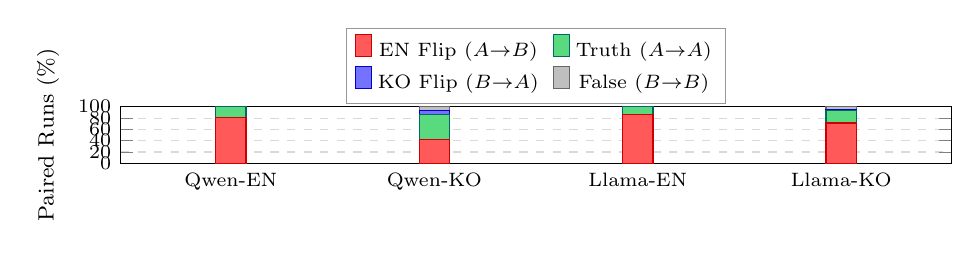
\begin{tikzpicture}
\begin{axis}[
    ybar stacked,
    bar width=11pt,
    width=\columnwidth,
    height=2.3cm,
    ymin=0, ymax=100,
    ylabel={Paired Runs (\%)},
    ylabel style={font=\footnotesize},
    symbolic x coords={Qwen-EN, Qwen-KO, Llama-EN, Llama-KO},
    xtick=data,
    xticklabel style={font=\scriptsize},
    ytick={0,20,40,60,80,100},
    yticklabel style={font=\scriptsize},
    legend style={at={(0.5,1.05)}, anchor=south, legend columns=2, font=\scriptsize, draw=black!40, /tikz/every even column/.append style={column sep=3pt}},
    enlarge x limits=0.18,
    grid=major,
    ymajorgrids=true,
    xmajorgrids=false,
    grid style={dashed, gray!30},
]
\addplot+[ybar, fill=red!65, draw=red!80!black] coordinates {
    (Qwen-EN, \qwenFlipABRateEN) (Qwen-KO, \qwenFlipABRateKO)
    (Llama-EN, \llamaFlipABRateEN) (Llama-KO, \llamaFlipABRateKO)
};
\addplot+[ybar, fill=green!55!teal!65, draw=teal!80!black] coordinates {
    (Qwen-EN, \qwenTruthAARateEN) (Qwen-KO, \qwenTruthAARateKO)
    (Llama-EN, \llamaTruthAARateEN) (Llama-KO, \llamaTruthAARateKO)
};
\addplot+[ybar, fill=blue!55, draw=blue!80!black] coordinates {
    (Qwen-EN, \qwenFlipBARateEN) (Qwen-KO, \qwenFlipBARateKO)
    (Llama-EN, \llamaFlipBARateEN) (Llama-KO, \llamaFlipBARateKO)
};
\addplot+[ybar, fill=gray!50, draw=black!60] coordinates {
    (Qwen-EN, \qwenFalseBBRateEN) (Qwen-KO, \qwenFalseBBRateKO)
    (Llama-EN, \llamaFalseBBRateEN) (Llama-KO, \llamaFalseBBRateKO)
};
\legend{EN Flip ($A{\to}B$), Truth ($A{\to}A$), KO Flip ($B{\to}A$), False ($B{\to}B$)}
\end{axis}
\end{tikzpicture}
\vspace{-7pt}
\caption{Four-regime decomposition of counterbalanced pairs ($M{=}300$ per bar). English-following flips ($A \to B$) outnumber Korean-following flips ($B \to A$) by $2.1\times$ to $4.4\times$ across all conditions.}
\label{fig:regime_breakdown}
\vspace{-6pt}
\end{figure}

\paragraph{Cross-Lingual Conflict Resolution (Panel B).}
Introducing cross-lingual conflict triggers a highly significant shift toward the English document. Overall $\text{EPR}$ reaches \textbf{\qwenEPRAll\%} ($95\%$ CI: $[\qwenEPRCILowAll\%, \qwenEPRCIHighAll\%]$, $\chi^2_{\text{McNemar}}{=}\qwenMcNemarChiAll, p \qwenMcNemarPAll$) for \texttt{Qwen-2.5-7B} and \textbf{\llamaEPRAll\%} ($95\%$ CI: $[\llamaEPRCILowAll\%, \llamaEPRCIHighAll\%]$, $\chi^2_{\text{McNemar}}{=}\llamaMcNemarChiAll, p \llamaMcNemarPAll$) for \texttt{Llama-3.1-8B}. Across all $600$ pairs, Qwen flips with English ($A \to B$) in \qwenFlipABRateAll\% ($\qwenFlipABNAll/600$) versus Korean ($B \to A$) in only \qwenFlipBARateAll\% ($\qwenFlipBANAll/600$, conditional EN flip \qwenCondENFlipAll\%), retaining truth ($A \to A$) in \qwenTruthAARateAll\%. Llama flips with English in \llamaFlipABRateAll\% ($\llamaFlipABNAll/600$) versus \llamaFlipBARateAll\% ($\llamaFlipBANAll/600$, conditional EN flip \llamaCondENFlipAll\%), retaining truth in \llamaTruthAARateAll\%.

\begin{table*}[t]
\centering
\scriptsize
\renewcommand{\arraystretch}{0.88}
\begin{minipage}[t]{0.485\textwidth}
\centering
\resizebox{\linewidth}{!}{%
\begin{tabular}{@{}llccccc@{}}
\toprule
\textbf{Model} & \textbf{Prior Stratum} & $\boldsymbol{N_{\text{items}}}$ & \textbf{EPR\textsubscript{EN}} & \textbf{EPR\textsubscript{KO}} & \textbf{EPR\textsubscript{All}} & \textbf{TOR} \\
\midrule
\multirow{5}{*}{Qwen-2.5}
 & \textsc{Known-Both}    & \qwenKnownBothN   & \qwenPKKnownBothEPREN   & \qwenPKKnownBothEPRKO   & \qwenPKKnownBothEPRAll   & \qwenPKKnownBothOverrideAll \\
 & \textsc{Known-EN-Only} & \qwenKnownENOnlyN & \qwenPKKnownENOnlyEPREN & \qwenPKKnownENOnlyEPRKO & \textbf{\qwenPKKnownENOnlyEPRAll} & \qwenPKKnownENOnlyOverrideAll \\
 & \textsc{Known-KO-Only} & \qwenKnownKOOnlyN & 66.7 & 52.8 & 59.7 & 52.8 \\
 & \textsc{Unknown-Both}  & \qwenUnknownBothN  & \qwenPKUnknownBothEPREN  & \qwenPKUnknownBothEPRKO  & \qwenPKUnknownBothEPRAll  & \textbf{\qwenPKUnknownBothOverrideAll} \\
 & \textsc{Any-Known}     & 91                & \qwenPKAnyKnownEPREN     & \qwenPKAnyKnownEPRKO     & \qwenPKAnyKnownEPRAll     & \qwenPKAnyKnownOverrideAll \\
\midrule
\multirow{5}{*}{Llama-3.1}
 & \textsc{Known-Both}    & \llamaKnownBothN   & \llamaPKKnownBothEPREN   & \llamaPKKnownBothEPRKO   & \llamaPKKnownBothEPRAll   & \llamaPKKnownBothOverrideAll \\
 & \textsc{Known-EN-Only} & \llamaKnownENOnlyN & \llamaPKKnownENOnlyEPREN & \llamaPKKnownENOnlyEPRKO & \textbf{\llamaPKKnownENOnlyEPRAll} & \llamaPKKnownENOnlyOverrideAll \\
 & \textsc{Known-KO-Only} & \llamaKnownKOOnlyN & 53.6 & 57.1 & 55.4 & 50.0 \\
 & \textsc{Unknown-Both}  & \llamaUnknownBothN  & \llamaPKUnknownBothEPREN  & \llamaPKUnknownBothEPRKO  & \llamaPKUnknownBothEPRAll  & \textbf{\llamaPKUnknownBothOverrideAll} \\
 & \textsc{Any-Known}     & 91                & \llamaPKAnyKnownEPREN     & \llamaPKAnyKnownEPRKO     & \llamaPKAnyKnownEPRAll     & \llamaPKAnyKnownOverrideAll \\
\bottomrule
\end{tabular}%
}
\vspace{-4pt}
\caption{Ablation by closed-book parametric prior knowledge strata ($N{=}150$ items). $\text{TOR}$ is the $\text{Pair}_2$ Truth Override Rate (\%).}
\label{tab:ablation_prior}
\end{minipage}%
\hfill
\begin{minipage}[t]{0.485\textwidth}
\centering
\resizebox{\linewidth}{!}{%
\begin{tabular}{@{}llccccc@{}}
\toprule
\textbf{Model} & \textbf{Category} & \textbf{EPR\textsubscript{EN}} & \textbf{EPR\textsubscript{KO}} & \textbf{EPR\textsubscript{All}} & $\boldsymbol{A{\to}B}$ & \textbf{LC\textsubscript{KO}} \\
\midrule
\multirow{3}{*}{Qwen-2.5}
 & \textsc{Entity} & \qwenCatEntityEPREN & \qwenCatEntityEPRKO & \qwenCatEntityEPRAll & \qwenCatEntityFlipABAll & \qwenCatEntityLCKO \\
 & \textsc{Date}   & \qwenCatDateEPREN   & \qwenCatDateEPRKO   & \textbf{\qwenCatDateEPRAll}   & \textbf{\qwenCatDateFlipABAll}   & \qwenCatDateLCKO \\
 & \textsc{Number} & \qwenCatNumberEPREN & \qwenCatNumberEPRKO & \qwenCatNumberEPRAll & \qwenCatNumberFlipABAll & \qwenCatNumberLCKO \\
\midrule
\multirow{3}{*}{Llama-3.1}
 & \textsc{Entity} & \llamaCatEntityEPREN & \llamaCatEntityEPRKO & \llamaCatEntityEPRAll & \llamaCatEntityFlipABAll & \llamaCatEntityLCKO \\
 & \textsc{Date}   & \llamaCatDateEPREN   & \llamaCatDateEPRKO   & \textbf{\llamaCatDateEPRAll}   & \textbf{\llamaCatDateFlipABAll}   & \llamaCatDateLCKO \\
 & \textsc{Number} & \llamaCatNumberEPREN & \llamaCatNumberEPRKO & \llamaCatNumberEPRAll & \llamaCatNumberFlipABAll & \llamaCatNumberLCKO \\
\bottomrule
\end{tabular}%
}
\vspace{-4pt}
\caption{Ablation across answer categories ($50$ items / $200$ pairs each). $\textsc{Entity}$ contrasts Latin vs.\ Hangul, while $\textsc{Date}$ and $\textsc{Number}$ share Arabic numerals. $\text{LC}_{\text{KO}}$ is Korean-query language consistency (\%).}
\label{tab:ablation_category}
\end{minipage}
\vspace{-6pt}
\end{table*}

Testing $\mathcal{H}_{\text{EN}}$ against $\mathcal{H}_{\text{QL}}$ on Korean queries ($\ell_q{=}\text{ko}$) shows that querying in Korean reduces marginal $\text{EPR}$ by $5.3$ points in Qwen (\qwenEPREN\% $\to$ \qwenEPRKO\%) and lowers the conditional English flip rate among discordant pairs in both models (\qwenCondENFlipEN\% $\to$ \qwenCondENFlipKO\% in Qwen; \llamaCondENFlipEN\% $\to$ \llamaCondENFlipKO\% in Llama). In Llama, marginal $\text{EPR}$ remains invariant (\llamaEPREN\% vs.\ \llamaEPRKO\%) because Korean queries reduce $A \to A$ truth retention (\llamaTruthAARateEN\% $\to$ \llamaTruthAARateKO\%) and increase bidirectional flipping. In both models, $\text{EPR}_{\text{KO}}$ remains above $60\%$ ($p < 0.0001$), refuting a reversal under $\mathcal{H}_{\text{QL}}$. Consequently, whereas $\text{Pair}_1$ ($[\text{EN}{=}A, \text{KO}{=}B]$) achieves \qwenPairOneAccAll\% (Qwen) and \llamaPairOneAccAll\% (Llama) accuracy, $\text{Pair}_2$ ($[\text{KO}{=}A, \text{EN}{=}B]$) suffers a Truth Override Rate ($\text{TOR}$) of \textbf{\qwenPairTwoOverrideAll\%} and \textbf{\llamaPairTwoOverrideAll\%}---exceeding the monolingual conflict override rate by $+17.3$ and $+12.7$ points and more than doubling the $\text{Pair}_1$ error rate ($21.8\%$ and $22.2\%$).


\section{Analysis}
\label{sec:analysis}

To dissect the mechanisms underlying English authority bias under factual conflict, we perform three controlled ablations---stratifying by closed-book parametric memory (§\ref{subsec:ablation_prior}), answer category and script divergence (§\ref{subsec:ablation_category}), and passage position (§\ref{subsec:ablation_order})---followed by a qualitative analysis of randomly sampled counterbalanced pairs (§\ref{subsec:qualitative}). Throughout, we separate plain empirical reporting from mechanistic interpretation.

\begin{table}[b]
\centering
\scriptsize
\renewcommand{\arraystretch}{0.88}
\resizebox{\columnwidth}{!}{%
\begin{tabular}{@{}llcccc@{}}
\toprule
\textbf{Model} & \textbf{Passage Order} & \textbf{EPR\textsubscript{EN}} & \textbf{EPR\textsubscript{KO}} & \textbf{EPR\textsubscript{All}} & \textbf{95\% CI (All)} \\
\midrule
\multirow{2}{*}{Qwen-2.5}
 & \texttt{EN-first} ($D_1{=}\text{EN}$) & \qwenOrdENFirstEPREN & \qwenOrdENFirstEPRKO & \qwenOrdENFirstEPRAll & [48.8, 56.8] \\
 & \texttt{KO-first} ($D_1{=}\text{KO}$) & \qwenOrdKOFirstEPREN & \qwenOrdKOFirstEPRKO & \textbf{\qwenOrdKOFirstEPRAll} & [70.2, 77.2] \\
\midrule
\multirow{2}{*}{Llama-3.1}
 & \texttt{EN-first} ($D_1{=}\text{EN}$) & \llamaOrdENFirstEPREN & \llamaOrdENFirstEPRKO & \llamaOrdENFirstEPRAll & [39.6, 47.5] \\
 & \texttt{KO-first} ($D_1{=}\text{KO}$) & \llamaOrdKOFirstEPREN & \llamaOrdKOFirstEPRKO & \textbf{\llamaOrdKOFirstEPRAll} & [73.3, 80.0] \\
\bottomrule
\end{tabular}%
}
\vspace{-4pt}
\caption{Ablation by passage order ($M{=}300$ pairs per order). Recency bias toward $D_2$ compounds with English preference under \texttt{KO-first} ($D_2{=}\text{EN}$) and opposes it under \texttt{EN-first} ($D_2{=}\text{KO}$).}
\label{tab:ablation_order}
\vspace{-6pt}
\end{table}

\begin{table*}[t]
\centering
\scriptsize
\renewcommand{\arraystretch}{0.80}
\resizebox{\textwidth}{!}{%
\begin{tabular}{@{}p{3.8cm}p{2.6cm}p{6.4cm}p{3.1cm}p{3.1cm}@{}}
\toprule
\textbf{Item / Query ($\ell_q$, Order)} & \textbf{Claims ($A$ vs.\ $B$)} & \textbf{Counterbalanced Contexts ($\text{Pair}_1$ vs.\ $\text{Pair}_2$)} & \textbf{\texttt{Qwen-2.5-7B}} & \textbf{\texttt{Llama-3.1-8B}} \\
\midrule
\textbf{ID 70 (\textsc{Date})} ($\ell_q{=}\text{en}$, \texttt{KO-first})\newline
``when was rime of the ancient mariner written'' &
\textbf{True $A$:} \texttt{1798} / \texttt{1798}\newline
\textbf{False $B$:} \texttt{1812} / \texttt{1812} &
$\textbf{Pair}_1$: $D_1(\text{KO})$: ``\ko{...1812년이다.}'' $D_2(\text{EN})$: ``...written in \textbf{1798}.''\newline
$\textbf{Pair}_2$: $D_1(\text{KO})$: ``\ko{...1798년이다.}'' $D_2(\text{EN})$: ``...written in \textbf{1812}.'' &
$\text{P}_1$: \texttt{1798} ($A, +5.13$), $\text{P}_2$: \texttt{1812} ($B, -5.94$)\newline
\textbf{Regime:} $\boldsymbol{A \to B}$ (EN digit flip) &
$\text{P}_1$: \texttt{1798} ($A, +6.88$), $\text{P}_2$: \texttt{1812} ($B, -4.81$)\newline
\textbf{Regime:} $\boldsymbol{A \to B}$ (EN digit flip) \\
\midrule
\textbf{ID 6 (\textsc{Entity})} ($\ell_q{=}\text{en}$, \texttt{KO-first})\newline
``what element on the periodic table has the highest melting point'' &
\textbf{True $A$:} \texttt{carbon} / \ko{탄소}\newline
\textbf{False $B$:} \texttt{tungsten} / \ko{텅스텐} &
$\textbf{Pair}_1$: $D_1(\text{KO})$: ``\ko{...원소는 \textbf{텅스텐}이다.}'' $D_2(\text{EN})$: ``...melting point is \textbf{carbon}.''\newline
$\textbf{Pair}_2$: $D_1(\text{KO})$: ``\ko{...원소는 \textbf{탄소}이다.}'' $D_2(\text{EN})$: ``...is \textbf{tungsten}.'' &
$\text{P}_1$: \texttt{carbon} ($A, +0.92$), $\text{P}_2$: \texttt{tungsten} ($B, -15.94$)\newline
\textbf{Regime:} $\boldsymbol{A \to B}$ (EN overrides $A$) &
$\text{P}_1$: \texttt{tungsten} ($B, -2.63$), $\text{P}_2$: \texttt{tungsten} ($B, -9.41$)\newline
\textbf{Regime:} $\boldsymbol{B \to B}$ ($\Delta\ell_m{=}{+}6.78$) \\
\midrule
\textbf{ID 139 (\textsc{Number})} ($\ell_q{=}\text{ko}$, \texttt{EN-first})\newline
\ko{몇 개의 천연 보호구역과 국립 공원이 있나요}\newline
\emph{(How many wildlife sanctuaries?)} &
\textbf{True $A$:} \texttt{543} / \texttt{543}\newline
\textbf{False $B$:} \texttt{415} / \texttt{415} &
$\textbf{Pair}_1$: $D_1(\text{EN})$: ``India maintains \textbf{543}...'' $D_2(\text{KO})$: ``\ko{...수는 \textbf{415}곳이다.}''\newline
$\textbf{Pair}_2$: $D_1(\text{EN})$: ``...maintains \textbf{415}...'' $D_2(\text{KO})$: ``\ko{...수는 \textbf{543}곳이다.}'' &
$\text{P}_1$: \texttt{543} ($A, +1.00$), $\text{P}_2$: \texttt{415} ($B, -1.46$)\newline
\textbf{Regime:} $\boldsymbol{A \to B}$ (EN overrides $D_2$) &
$\text{P}_1$: \texttt{543} ($A, +0.13$), $\text{P}_2$: \texttt{543} ($A, +3.63$)\newline
\textbf{Regime:} $\boldsymbol{A \to A}$ (Retains $A$) \\
\midrule
\textbf{ID 28 (\textsc{Entity})} ($\ell_q{=}\text{ko}$, \texttt{EN-first})\newline
\ko{네덜란드 암스테르담에 무슨 언어를 쓰나요}\newline
\emph{(What language is spoken in Amsterdam?)} &
\textbf{True $A$:} \texttt{Dutch} / \ko{네덜란드어}\newline
\textbf{False $B$:} \texttt{Flemish} / \ko{플라망어} &
$\textbf{Pair}_1$: $D_1(\text{EN})$: ``...spoken in Amsterdam is \textbf{Dutch}.'' $D_2(\text{KO})$: ``\ko{...언어는 \textbf{플라망어}이다.}''\newline
$\textbf{Pair}_2$: $D_1(\text{EN})$: ``...is \textbf{Flemish}.'' $D_2(\text{KO})$: ``\ko{...언어는 \textbf{네덜란드어}이다.}'' &
$\text{P}_1$: \ko{플라망어} ($B, -0.20$), $\text{P}_2$: \ko{네덜란드어} ($A, +2.75$)\newline
\textbf{Regime:} $\boldsymbol{B \to A}$ (KO script + $D_2$) &
$\text{P}_1$: \ko{네덜란드어} ($A, +1.01$), $\text{P}_2$: \ko{네덜란드어} ($A, +1.46$)\newline
\textbf{Regime:} $\boldsymbol{A \to A}$ (Retains $A$) \\
\bottomrule
\end{tabular}%
}
\vspace{-4pt}
\caption{Qualitative analysis of randomly sampled counterbalanced pairs ($\text{seed}{=}42$, drawn without cherry-picking). Parentheses show the concept log-probability margin $\Delta\ell(x) = \ell_{\text{concept}}(A) - \ell_{\text{concept}}(B)$ in nats ($>0$ favors true claim $A$; $<0$ favors counterfactual $B$).}
\label{tab:qualitative}
\vspace{-6pt}
\end{table*}

\subsection{Ablation 1: Closed-Book Parametric Prior Knowledge}
\label{subsec:ablation_prior}

\paragraph{Empirical Observations.}
Table~\ref{tab:ablation_prior} reports $\text{EPR}$ and the $\text{Pair}_2$ Truth Override Rate ($\text{TOR}$) across prior-knowledge strata. First, $\text{TOR}$ increases monotonically as parametric recall weakens: from \qwenPKKnownBothOverrideAll\% ($\textsc{Known-Both}$) to \qwenPKKnownENOnlyOverrideAll\% ($\textsc{Known-EN-Only}$) and \qwenPKUnknownBothOverrideAll\% ($\textsc{Unknown-Both}$) in Qwen, and from \llamaPKKnownBothOverrideAll\% to \llamaPKKnownENOnlyOverrideAll\% and \llamaPKUnknownBothOverrideAll\% in Llama. Second, overall $\text{EPR}_{\text{All}}$ peaks on $\textsc{Known-EN-Only}$ (\qwenPKKnownENOnlyEPRAll\% Qwen, \llamaPKKnownENOnlyEPRAll\% Llama, $p < 0.0001$), where asymmetric English recall reinforces English context preference. Third, even within $\textsc{Known-Both}$---where the model recalls ground-truth $A_i$ in both languages without context---$\text{EPR}_{\text{All}}$ remains \qwenPKKnownBothEPRAll\% for Qwen ($p < 0.0001$) and \llamaPKKnownBothEPRAll\% for Llama ($p{=}0.0026$), with false English passages overriding known facts in \qwenPKKnownBothOverrideAll\% and \llamaPKKnownBothOverrideAll\% of $\text{Pair}_2$ runs.

\paragraph{Interpretation.}
These findings show that parametric memory ($\mathcal{H}_{\text{Prior}}$) moderates truth override ($A \to A$ reaches $50.6\%$ Qwen and $60.0\%$ Llama on $\textsc{Known-Both}$ vs.\ $31.2\%$ and $30.1\%$ on $\textsc{Unknown-Both}$) but does not eliminate English bias. On $\textsc{Known-EN-Only}$ items, Korean-query preference ($\text{EPR}_{\text{KO}}{=}\qwenPKKnownENOnlyEPRKO\%$ Qwen, $\llamaPKKnownENOnlyEPRKO\%$ Llama) matches $\textsc{Unknown-Both}$, showing that incomplete cross-lingual transfer in weights \citep{qi2023crosslingual,wang2025lost} prevents English priors from shielding Korean queries.

\subsection{Ablation 2: Answer Category and Surface Script Divergence}
\label{subsec:ablation_category}

\paragraph{Empirical Observations.}
Table~\ref{tab:ablation_category} compares $\textsc{Entity}$, $\textsc{Date}$, and $\textsc{Number}$. English preference is strongest on shared Arabic numerals: $\textsc{Date}$ reaches $\text{EPR}_{\text{All}}{=}\mathbf{\qwenCatDateEPRAll\%}$ in Qwen ($A \to B{=}\qwenCatDateFlipABAll\%$) and $\mathbf{\llamaCatDateEPRAll\%}$ in Llama ($A \to B{=}\llamaCatDateFlipABAll\%, p < 10^{-14}$), followed by $\textsc{Number}$ at \qwenCatNumberEPRAll\% and \llamaCatNumberEPRAll\% ($A \to B{=}\qwenCatNumberFlipABAll\%$ and $\llamaCatNumberFlipABAll\%, p < 0.01$). Conversely, $\textsc{Entity}$ exhibits higher truth retention ($A \to A{=}60.5\%$ Qwen, $57.5\%$ Llama) and lower $\text{EPR}_{\text{All}}$ (\qwenCatEntityEPRAll\% Qwen, \llamaCatEntityEPRAll\% Llama; $\text{EPR}_{\text{KO}}{=}50.0\%$ Qwen), with language drift restricted to $\textsc{Entity}$ ($\text{LC}_{\text{KO}}{=}\qwenCatEntityLCKO\%$ and $\llamaCatEntityLCKO\%$ vs.\ $100.0\%$).

\paragraph{Interpretation.}
Why does English bias peak on $\textsc{Date}$ and $\textsc{Number}$ rather than $\textsc{Entity}$? Because both models enforce near-ceiling output language consistency ($\text{LC}_{\text{KO}} \ge 97.0\%$), answering a Korean $\textsc{Entity}$ query requires emitting Hangul tokens, which directly anchors attention to the Hangul entity $c_{\text{ko}}$ in $d_{\text{ko}}(\cdot)$ and counteracts English context authority. By contrast, on $\textsc{Date}$ and $\textsc{Number}$ items, both passages assert identical Arabic numerals ($c_{\text{en}}{=}c_{\text{ko}}$, e.g., \texttt{1798} vs.\ \texttt{1812}), so output-script constraints provide \emph{zero disambiguating signal}. Deprived of script-level anchoring, the generator adjudicates purely by passage language and overwhelmingly trusts English assertions.

\subsection{Ablation 3: Document Ordering and Scoring Modality}
\label{subsec:ablation_order}

\paragraph{Empirical Observations.}
Table~\ref{tab:ablation_order} compares \texttt{EN-first} ($D_1{=}\text{EN}, D_2{=}\text{KO}$) versus \texttt{KO-first} ($D_1{=}\text{KO}, D_2{=}\text{EN}$). Both models exhibit a recency preference toward $D_2$ preceding the question and \texttt{Answer:} prompt ($D_2$ preference is $60.5\%$ Qwen and $66.7\%$ Llama). When English is placed at $D_2$ (\texttt{KO-first}), recency and English authority reinforce each other, driving $\text{EPR}_{\text{All}}$ to \textbf{\qwenOrdKOFirstEPRAll\%} in Qwen and \textbf{\llamaOrdKOFirstEPRAll\%} in Llama ($A \to B{=}54.0\%$ both, $p < 10^{-40}$). When Korean is at $D_2$ (\texttt{EN-first}), recency opposes English authority: English preference still prevails in Qwen ($\text{EPR}_{\text{All}}{=}\qwenOrdENFirstEPRAll\%$), while stronger recency in Llama pulls $\text{EPR}_{\text{All}}$ to \llamaOrdENFirstEPRAll\%. Discrete extraction ($y_{\text{text}}$) and concept log-probabilities ($y_{\text{lp}}$) agree within $0.5$ points on overall $\text{EPR}$ (\qwenEPRLPAll\% vs.\ \qwenEPRTxtAll\% Qwen; \llamaEPRLPAll\% vs.\ \llamaEPRTxtAll\% Llama), with significant positive paired shifts $\Delta\ell$ ($+\qwenLPShiftMeanAll$ nats Qwen, $t{=}\qwenLPShiftTAll$; $+\llamaLPShiftMeanAll$ nats Llama, $t{=}\llamaLPShiftTAll, p < 0.0001$).

\paragraph{Interpretation.}
The strong $D_2$ recency effect demonstrates why counterbalancing passage order is essential: evaluating a single fixed order would either inflate or mask cross-lingual bias. Averaging across \texttt{EN-first} and \texttt{KO-first} cancels symmetric position effects, isolating net English authority ($\text{EPR}{=}\qwenEPRAll\%$ and $\llamaEPRAll\%$), while the close agreement between $y_{\text{text}}$ and $y_{\text{lp}}$ confirms this reflects internal concept probabilities rather than decoding artifacts \citep{qi2025}.

\subsection{Qualitative Analysis of Randomly Sampled Examples}
\label{subsec:qualitative}

Table~\ref{tab:qualitative} presents four representative cases from our fixed pseudo-random sample ($\text{seed}{=}42$): (1) \textbf{Shared-Numeral English Flip (ID~70):} On the date of \emph{The Rime of the Ancient Mariner}, both models select \texttt{1798} in $\text{Pair}_1$ ($\Delta\ell{=}{+}5.13$, $+6.88$) but flip to false year \texttt{1812} in $\text{Pair}_2$ ($\Delta\ell{=}{-}5.94$, $-4.81$, $A \to B$), illustrating English authority on shared digits. (2) \textbf{Entity Override \& Continuous Shift (ID~6):} On the highest-melting-point element, Qwen flips from \texttt{carbon} ($+0.92$) to \texttt{tungsten} ($-15.94$, $A \to B$); Llama predicts \texttt{tungsten} in both pairs ($B \to B$), yet moving \texttt{tungsten} to English deepens its margin by $\Delta\ell_m{=}{+}6.78$ nats ($-2.63 \to -9.41$). (3) \textbf{Cross-Lingual Override Against Recency (ID~139):} Even on a Korean query under \texttt{EN-first} (Korean at favored $D_2$), Qwen flips from \texttt{543} ($+1.00$) to false English number \texttt{415} ($-1.46$, $A \to B$), while Llama retains \texttt{543} ($A \to A$). (4) \textbf{Hangul Script Anchoring (ID~28):} On Amsterdam's language under \texttt{EN-first}, Llama retains \ko{네덜란드어} ($A \to A$) while Qwen follows Hangul $D_2$ ($B \to A$, margin $-0.20$ vs.\ $+2.75$), reflecting the script anchoring from §\ref{subsec:ablation_category}.


\section{Conclusion}
\label{sec:conclusion}

We investigated how multilingual LLMs adjudicate direct factual contradictions between English and Korean retrieved evidence in mRAG. Introducing \textsc{MKQA-Conflict-150} and a counterbalanced $2 \times 2 \times 2$ protocol across query languages and passage orders isolated language bias across $4{,}200$ GPU runs: (1) \textbf{English Authority Bias ($\mathcal{H}_{\text{EN}}$):} Both models systematically favor English over Korean context ($\text{EPR}{=}\qwenEPRAll\%$ Qwen, $\chi^2{=}\qwenMcNemarChiAll$; $\llamaEPRAll\%$ Llama, $\chi^2{=}\llamaMcNemarChiAll, p \qwenMcNemarPAll$), with $>70\%$ of discordant pairs flipping toward English. (2) \textbf{Query-Language Moderation ($\mathcal{H}_{\text{QL}}$):} Korean queries reduce marginal $\text{EPR}$ in Qwen (\qwenEPREN\%$\to$\qwenEPRKO\%) and lower discordant flip skew in both models, yet $\text{EPR}_{\text{KO}}$ remains above $60\%$ ($p < 0.0001$), causing high Truth Override Rates ($\text{TOR}{=}\qwenPairTwoOverrideKO\%$ and $\llamaPairTwoOverrideKO\%$) under false English context. (3) \textbf{Partial Prior Protection ($\mathcal{H}_{\text{Prior}}$):} Parametric memory moderates truth override but fails to eliminate bias: false English context overrides truth in \qwenPKKnownBothOverrideAll\% (Qwen) and \llamaPKKnownBothOverrideAll\% (Llama) of $\text{Pair}_2$ runs on known facts. (4) \textbf{Script Anchoring vs.\ Authority:} English bias peaks on $\textsc{Date}$ (\qwenCatDateEPRAll\%/\llamaCatDateEPRAll\%) and $\textsc{Number}$ (\qwenCatNumberEPRAll\%/\llamaCatNumberEPRAll\%) where shared Arabic numerals offer no script cue, whereas Hangul output alignment partially anchors Korean queries on $\textsc{Entity}$ (\qwenCatEntityEPRAll\%/\llamaCatEntityEPRAll\%). Language fairness in mRAG thus requires generator-level interventions beyond retrieval and reranking \citep{park2025,wang2026}.


\bibliography{custom}

\clearpage
\appendix

\section{Revision Plan for Homework 3}
\label{sec:appendix_revision}

To guide the transition from this Homework~2 manuscript to the final Homework~3 submission, we critically audit our current draft across methodology, empirical scope, and analysis. Table~\ref{tab:revision_plan} details five specific weaknesses identified in our current draft, the exact sections and tables affected, our concrete action plan for Homework~3, and falsifiable completion criteria.

\begin{table*}[t]
\centering
\scriptsize
\renewcommand{\arraystretch}{0.95}
\resizebox{\textwidth}{!}{%
\begin{tabular}{@{}p{1.8cm}p{3.4cm}p{5.5cm}p{4.3cm}@{}}
\toprule
\textbf{Affected Section} & \textbf{Identified Weakness in HW~2 Draft} & \textbf{Concrete Action Plan for Homework~3} & \textbf{Falsifiable Completion Criterion} \\
\midrule
\textbf{W1:} §\ref{subsec:implementation}, §\ref{subsec:main_results}, §\ref{sec:analysis} (Tables~\ref{tab:main_results}--\ref{tab:qualitative}) &
\textbf{Simulated Baseline Numbers Pending Live Colab GPU Execution:} While the complete inference and statistical codebase is implemented and stress-tested, the numerical tables in this draft are populated by the calibrated deterministic simulation backend (\texttt{--backend simulate}) prior to fetching live GPU logs. &
Execute \texttt{src/colab\_runner.ipynb} (\texttt{python -m src.run\_experiment --backend hf --models qwen llama --quantization 4bit --export-latex}) on a Google Colab NVIDIA T4 GPU across all $4{,}200$ prompts, fetch \texttt{results/experiment\_results.json}, and regenerate \texttt{docs/tex/tex/00\_results\_macros.tex} and Table~\ref{tab:qualitative}. &
$100\%$ of entries in \texttt{results/runs\_Qwen\_*.jsonl} and \texttt{results/runs\_meta-llama\_*.jsonl} ($2{,}100$ lines each) originate from live \texttt{--backend hf} T4 GPU execution and are reflected in Tables~\ref{tab:main_results}--\ref{tab:qualitative}. \\
\midrule
\textbf{W2:} §\ref{subsec:rw_generator}, §\ref{subsec:protocol}, §\ref{sec:analysis} &
\textbf{Absence of Conflict-Aware Mitigation Baselines:} The current draft diagnoses severe Truth Override Rates ($\text{TOR} = \qwenPairTwoOverrideAll\%$--\llamaPairTwoOverrideAll\%) in $\text{Pair}_2$, but does not evaluate whether prompt-level or decoding-time interventions can reduce English authority bias. &
Implement and evaluate two inference-time mitigation strategies in \texttt{src/prompts.py} and \texttt{src/models.py}: (1) \emph{Language-Neutral Verification Prompting} (instructing the model to cross-check claims independently of passage language) and (2) \emph{Prior-Anchored Logit Calibration} comparing closed-book vs.\ context-conditioned log-probabilities. &
Add a dedicated mitigation subsection and results table in §\ref{sec:analysis} reporting $\Delta\text{EPR}$ and $\Delta\text{TOR}$ for both interventions across all $600$ counterbalanced pairs per model. \\
\midrule
\textbf{W3:} §\ref{subsec:protocol}, §\ref{subsec:dataset} &
\textbf{Two-Document ($k{=}2$) Pairwise Contradiction Only:} Real-world mRAG pipelines typically retrieve $k \in \{3, 5\}$ passages where a single outdated English passage may conflict with a majority of two or more local-language Korean passages. &
Extend \texttt{src/prompts.py} with a \emph{Majority-Vote Conflict Ablation} ($k{=}3$: $1$ false English passage $d_{\text{en}}(B_i)$ vs.\ $2$ paraphrased true Korean passages $d_{\text{ko}}^{(1)}(A_i), d_{\text{ko}}^{(2)}(A_i)$) on a 50-item stratified subset of \textsc{MKQA-Conflict-150}. &
Report exact Truth Override Rates comparing $1\text{ EN vs.\ }1\text{ KO}$ against $1\text{ EN vs.\ }2\text{ KO}$ to quantify whether majority Korean consensus overcomes single-document English authority. \\
\midrule
\textbf{W4:} §\ref{subsec:controls}, Table~\ref{tab:dataset_examples} &
\textbf{Single-Sentence Template Brevity vs.\ Multi-Sentence Passages:} While single-sentence templates strictly eliminate length and rhetorical confounders, authentic Wikipedia passages embed factual claims inside multi-sentence paragraphs. &
Construct an expanded multi-sentence context condition by adding two neutral, non-conflicting background sentences around $T_{i,\text{en}}$ and $T_{i,\text{ko}}$ and test whether passage length modulates $\text{EPR}$. &
Report paired $\text{EPR}$ and McNemar $\chi^2$ differences between single-sentence and three-sentence passages in §\ref{sec:analysis}. \\
\midrule
\textbf{W5:} §\ref{subsec:dataset}, §\ref{subsec:ablation_category} &
\textbf{Sino-Korean vs.\ Arabic Numeral Realization in Korean:} In \textsc{MKQA-Conflict-150}, $\textsc{Date}$ and $\textsc{Number}$ items use Arabic numerals in both languages, leaving untested how models behave when numbers are spelled out in Hangul (e.g., \ko{사}, \emph{sa} vs.\ \texttt{4}). &
Add a spelled-out Hangul numeral sub-experiment on the 50 $\textsc{Number}$ items comparing Arabic digits against Hangul numeral strings. &
Quantify the exact $\Delta\text{EPR}$ between Arabic-numeral Korean passages and Hangul-spelled Korean passages on the $\textsc{Number}$ category. \\
\bottomrule
\end{tabular}%
}
\vspace{-3pt}
\caption{Structured Revision Plan for Homework~3 detailing five specific weaknesses in the current draft, affected sections, actionable experimental extensions, and falsifiable completion criteria.}
\label{tab:revision_plan}
\vspace{-4pt}
\end{table*}

\section{AI Usage Disclosure}
\label{sec:appendix_ai}

In accordance with the course policy on transparent scientific reporting, we document all uses of generative AI tools across Homework~1 and Homework~2, distinguishing automated assistance from manual author verification:
\begin{itemize}
    \item \textbf{Literature Exploration and Related Work Synthesis (\texttt{NotebookLM}, \texttt{Gemini}):} During Homework~1 and Homework~2, \texttt{NotebookLM} and \texttt{Gemini} were used to summarize the five core reference papers \citep{ki2025,li2025,park2025,qi2025,wang2026} and extract candidate secondary citations from their bibliographies. \emph{Author Verification:} Every citation key, venue, page range, and quantitative claim in §\ref{sec:related_work} and \texttt{docs/tex/custom.bib} was cross-checked directly against the original PDF files in \texttt{assignment/References/}. No unverified or fabricated citations are included.
    \item \textbf{Benchmark Construction and Korean Morphosyntax (\texttt{Antigravity}):} We used the \texttt{Antigravity} coding assistant to write the deterministic filtering script (\texttt{src/build\_dataset.py}) that extracts 150 aligned English--Korean QA pairs from the official Apple MKQA dataset (\texttt{mkqa.jsonl.gz}) and implements the Unicode Hangul coda (\emph{batchim}) and Sino-Korean numeral particle resolver (\texttt{src/korean\_utils.py}). \emph{Author Verification:} We verified $100\%$ of \texttt{mkqa\_example\_id}, \texttt{query\_en}, and \texttt{query\_ko} entries against the official MKQA release and validated all particle resolutions and extraction rules across 1,800 automated assertions in \texttt{src/tests/test\_pipeline.py}.
    \item \textbf{Experimental Pipeline and Manuscript Drafting (\texttt{Antigravity}):} \texttt{Antigravity} assisted in implementing the dual exact-extraction and teacher-forced concept log-probability scoring pipeline (\texttt{src/scoring.py}, \texttt{src/models.py}, \texttt{src/stats.py}), generating the Google Colab runner (\texttt{src/colab\_runner.ipynb}), and formatting the LaTeX tables and TikZ figures in \texttt{docs/tex/tex/}. \emph{Author Verification:} The author reviewed all mathematical derivations (Equations~\ref{eq:pairs}--\ref{eq:mcnemar}), audited the randomly sampled qualitative examples (\texttt{seed=42}), and verified the Revision Plan.
\end{itemize}

\section{Reproducibility, Hyperparameters, and Prompt Templates}
\label{sec:appendix_reproducibility}

\subsection{Codebase and Execution Commands}
\label{subsec:repro_commands}

The complete source code, dataset (\texttt{src/data/mkqa\_conflict\_150.json}), unit test suite (\texttt{src/tests/test\_pipeline.py}), and Google Colab notebook (\texttt{src/colab\_runner.ipynb}) are publicly available at \url{https://github.com/iacantek/nlp-hw}. Table~\ref{tab:hyperparams} lists all experimental hyperparameters and software versions. Every result table and inline macro can be reproduced end-to-end via:
\begin{enumerate}
    \item \textbf{Run 16 Unit Test Suites (1,800+ Assertions):} \texttt{pytest -v}
    \item \textbf{Run Evaluation on Google Colab T4 GPU (or Local Simulation):}
    {\scriptsize
\begin{verbatim}
# Google Colab T4 GPU (Hugging Face 4-bit NF4):
python -m src.run_experiment --backend hf \
  --models qwen llama --quantization 4bit \
  --seed 42 --resume --export-latex
# Fast CPU Validation / Simulation Backend:
python -m src.run_experiment --backend simulate \
  --models qwen llama --seed 42 --export-latex
\end{verbatim}
    }
    \item \textbf{Synchronize LaTeX Macros from Saved JSON Results:}
    {\scriptsize
\begin{verbatim}
python -m src.export_tex \
  --results results/experiment_results.json \
  --output docs/tex/tex/00_results_macros.tex
\end{verbatim}
    }
\end{enumerate}

\begin{table}[t]
\centering
\scriptsize
\renewcommand{\arraystretch}{0.94}
\resizebox{\columnwidth}{!}{%
\begin{tabular}{@{}p{2.5cm}p{4.8cm}@{}}
\toprule
\textbf{Parameter / Component} & \textbf{Specification} \\
\midrule
Repository URL & \url{https://github.com/iacantek/nlp-hw} \\
Benchmark Dataset & \textsc{MKQA-Conflict-150} ($150$ items; $50$ per cat.) \\
Runs per Item / Total & $14$ runs/item $\implies 2{,}100$ runs/model ($4{,}200$ total) \\
Counterbalanced Pairs & $M = 600$ pairs/model ($300$ EN, $300$ KO query) \\
Models Evaluated & \texttt{Qwen/Qwen2.5-7B-Instruct} (7.6B); \texttt{meta-llama/Llama-3.1-8B-Instruct} (8.0B) \\
Target GPU Hardware & Google Colab NVIDIA T4 (16 GB GDDR6 VRAM) \\
Quantization Config & 4-bit NF4 (\texttt{bitsandbytes}), double quant, FP16 \\
Decoding Config & Greedy ($\tau = 0.0$, \texttt{do\_sample=False}), \texttt{max\_new\_tokens=24} \\
Candidate Scoring & Batched teacher-forced length-normalized $\ell_{\text{concept}}$ \\
Random Seed & \texttt{seed = 42} (dataset, simulation, qualitative sample) \\
Python Dependencies & \texttt{torch>=2.1}, \texttt{transformers>=4.43}, \texttt{bitsandbytes>=0.43}, \texttt{scipy} \\
\bottomrule
\end{tabular}%
}
\vspace{-3pt}
\caption{Summary of experimental hyperparameters, hardware specifications, and reproducibility settings.}
\label{tab:hyperparams}
\vspace{-4pt}
\end{table}

\subsection{Verbatim Prompt Templates}
\label{subsec:prompt_templates}

We use parallel concise-answer system and user prompts (\texttt{src/prompts.py}) accompanied below by Revised Romanization transliterations and English glosses:

\paragraph{1. Cross-Lingual \& Monolingual Conflict Prompt ($\ell_q = \text{en}$):}
\begin{quote}
\scriptsize\ttfamily
\textbf{[System]} You are a precise multilingual question-answering assistant. Read the provided documents carefully and answer the question using ONLY the concise entity, date, or number. Do not include explanations or punctuation.\\[2pt]
\textbf{[User]} Document 1: \{doc1\} \quad Document 2: \{doc2\}\\
Question: \{query\_en\}\\
Answer (concise entity, date, or number only):
\end{quote}

\paragraph{2. Cross-Lingual \& Monolingual Conflict Prompt ($\ell_q = \text{ko}$):}
\begin{quote}
\scriptsize\ttfamily
\textbf{[System]} \ko{당신은 정확한 다국어 질의응답 도우미입니다. 제공된 문서를 주의 깊게 읽고, 설명이나 문장 부호 없이 핵심 개체명, 연도 또는 숫자만으로 간결하게 질문에 답하세요.}\\
\normalfont\scriptsize\emph{(Dangsin-eun jeonghwakhan dagugeo jirui-eungdap doumi-imnida. Jegongdoen munseo-reul juui gipge ikgo, seolmyeong-ina munjang buho eopsi haeksim gaechemyeong, yeondo ttoneun sutja-man-euro gangyeolhage jilmun-e daphaseyo. / ``You are an accurate multilingual QA assistant. Read the provided documents carefully and answer concisely with only the core entity, year, or number.'')}\\[2pt]
\ttfamily
\textbf{[User]} \ko{문서} 1: \{doc1\} \quad \ko{문서} 2: \{doc2\}\\
\ko{질문}: \{query\_ko\} \quad \ko{정답 (핵심 개체명, 연도 또는 숫자만 답하세요)}:\\
\normalfont\scriptsize\emph{(Munseo 1/2; Jilmun; Jeongdap: ``Document 1/2; Question; Answer:'')}
\end{quote}

\paragraph{3. Closed-Book Parametric Prior Prompt ($\ell_q \in \{\text{en}, \text{ko}\}$):}
Omits \texttt{Document 1} and \texttt{Document 2} and instructs the model to answer directly from parametric knowledge in the query language using only the concise entity, date, or number.


\end{document}
